\documentclass[a4paper,11pt]{article}
\usepackage[utf8]{inputenc}
\usepackage{cmap}
\usepackage[T1]{fontenc}
\usepackage{lmodern}
\usepackage{microtype}
\usepackage[margin=2.5cm]{geometry}
\usepackage{amsmath,amssymb,bm}
\usepackage{graphicx}
\usepackage[american]{circuitikz}
\usetikzlibrary{arrows.meta,positioning,calc,shapes.geometric}
\usepackage{booktabs}
\usepackage[hidelinks]{hyperref}
\setlength{\emergencystretch}{1.5em}

\newcommand{\La}{L_{\mathrm{arm}}}
\newcommand{\sgn}{\operatorname{sgn}}

\begin{document}

%======================================================================
\section{Mathematical Model For Furuta Pendulum}
%======================================================================

\begin{figure}[h]
  \centering
  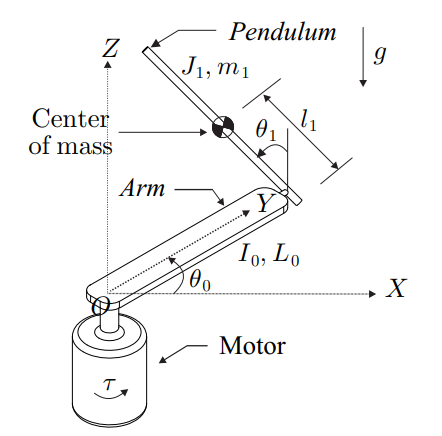
\includegraphics[width=0.45\textwidth]{furuta_fig.png}
  \caption{Furuta Pendulum. The symbols in the figure correspond to the text as
  $I_0 \to J_0$, $L_0 \to \La$, $m_1 \to m$, $l_1 \to L_p$ and $\tau \to T_m$.}
  \label{fig:furuta}
\end{figure}

\subsection{Rotary Arm}
Since the equations of motion of our system will be derived with the Lagrangian method, the kinetic and potential energies of each body are needed. The rotary arm only rotates about the vertical motor axis, so its kinetic energy is
\begin{equation}
  T_0 = \frac{1}{2} J_0 \dot\theta_0^2 ,
\end{equation}
where $J_0$ is the moment of inertia of the arm and its hub about the motor axis.

The inertia of the motor rotor and gearbox is not included here, since it is added later through the motor model (see section~\ref{sec:motor}).

Since the arm rotates in a horizontal plane and its height never changes, the plane of the arm is taken as the reference. Therefore, its gravitational potential energy is zero:
\begin{equation}
  U_0 = 0
\end{equation}

\subsection{Pendulum}
The pendulum is modeled using its mass $m$, located at a distance $L_p$ from the pivot, together with its moment of inertia $J_1$ about an axis through its center of mass perpendicular to the pendulum.

The arm length, from the motor axis to the pendulum pivot, is denoted by $\La$.

The two generalized coordinates of our system are:
\begin{itemize}
  \item $\theta_0$: rotation angle of the horizontal arm about the vertical axis.
  \item $\theta_1$: pendulum angle measured from the upright vertical position.
\end{itemize}

To find the kinetic energy of the pendulum, the velocity of its center of mass is needed, so its position is written first in the inertial frame (see Figure~\ref{fig:furuta}):
\begin{equation}
\begin{aligned}
  x_x &= \La \cos\theta_0 - L_p \sin\theta_1 \sin\theta_0 ,\\
  x_y &= \La \sin\theta_0 + L_p \sin\theta_1 \cos\theta_0 ,\\
  x_z &= L_p \cos\theta_1 .
\end{aligned}
\label{eq:pos}
\end{equation}

\subsubsection{Velocity of the Pendulum Center of Mass}
Differentiating the position coordinates of equation~\ref{eq:pos} with respect to time gives:
\begin{equation}
\begin{aligned}
  \dot x_x = {}& -\La \sin\theta_0\,\dot\theta_0\\
  & - L_p \cos\theta_1 \sin\theta_0\,\dot\theta_1\\
  & - L_p \sin\theta_1 \cos\theta_0\,\dot\theta_0 ,
\end{aligned}
\end{equation}
\begin{equation}
\begin{aligned}
  \dot x_y = {}& \La \cos\theta_0\,\dot\theta_0\\
  & + L_p \cos\theta_1 \cos\theta_0\,\dot\theta_1\\
  & - L_p \sin\theta_1 \sin\theta_0\,\dot\theta_0 ,
\end{aligned}
\end{equation}
\begin{equation}
  \dot x_z = -L_p \sin\theta_1\,\dot\theta_1 .
\end{equation}
Since the translational kinetic energy depends only on the speed, the squared magnitude of the velocity is needed:
\begin{equation}
  v^2 = \dot x_x^2 + \dot x_y^2 + \dot x_z^2 .
\end{equation}
Expanding and simplifying this expression (using MATLAB's symbolic toolbox) gives:
\begin{equation}
\begin{aligned}
  \therefore\; v^2 = {}& \La^2 \dot\theta_0^2 + L_p^2 \dot\theta_1^2\\
  & + L_p^2 \dot\theta_0^2 \sin^2\theta_1\\
  & + 2 \La L_p \dot\theta_0 \dot\theta_1 \cos\theta_1 .
\end{aligned}
\label{eq:v2}
\end{equation}
Equation~\ref{eq:v2} includes the full three-dimensional motion of the pendulum's center of mass. Its last term couples the two rotations, so the speed of the pendulum depends on the motion of both joints at the same time.

\subsubsection{Kinetic Energy of the Pendulum}
Since the pendulum also rotates while it moves, its kinetic energy has a rotational part as well as a translational one.

The angular velocity of the pendulum is the sum of the arm rotation $\dot\theta_0$ about the vertical axis and the pendulum rotation $\dot\theta_1$ about the arm axis. Resolving it along the principal axes of the pendulum gives:
\begin{itemize}
  \item $\dot\theta_1$ about the arm axis, which is perpendicular to the pendulum;
  \item $\dot\theta_0 \sin\theta_1$ about the axis perpendicular to both the arm and the pendulum;
  \item $\dot\theta_0 \cos\theta_1$ about the long axis of the pendulum.
\end{itemize}
Since the pendulum is a thin rod, it will be treated as a slender rod, so its moment of inertia about its long axis is neglected and $J_1$ applies to both perpendicular axes. Therefore, the rotational kinetic energy of the pendulum is:
\begin{equation}
  T_{\mathrm{rotational}} = \frac{1}{2} J_1 \left(\dot\theta_1^2 + \dot\theta_0^2 \sin^2\theta_1\right).
  \label{eq:Trot}
\end{equation}
The translational kinetic energy of the pendulum's mass is:
\begin{equation}
  T_{\mathrm{translational}} = \frac{1}{2} m v^2 .
\end{equation}
Substituting the squared speed from equation~\ref{eq:v2} gives:
\begin{equation}
  T_{\mathrm{translational}} = \frac{1}{2} m \left[\left(\dot\theta_0 \La\right)^2 + \left(\dot\theta_1 L_p\right)^2 + \left(\dot\theta_0 L_p \sin\theta_1\right)^2 + 2 L_p \La \dot\theta_0 \dot\theta_1 \cos\theta_1\right]
\end{equation}
and expanding the terms yields:
\begin{equation}
\begin{aligned}
  T_{\mathrm{translational}} = {}& \frac{1}{2} m \La^2 \dot\theta_0^2 + \frac{1}{2} m L_p^2 \dot\theta_1^2\\
  & + \frac{1}{2} m L_p^2 \dot\theta_0^2 \sin^2\theta_1\\
  & + m \La L_p \dot\theta_0 \dot\theta_1 \cos\theta_1 .
\end{aligned}
\end{equation}
By adding the rotational kinetic energy (equation~\ref{eq:Trot}) to the translational one, the total kinetic energy of the pendulum is:
\begin{equation}
\begin{aligned}
  \therefore\; T_1 = {}& \frac{1}{2} m \La^2 \dot\theta_0^2 + \frac{1}{2}\left(J_1 + m L_p^2\right)\dot\theta_1^2\\
  & + \frac{1}{2}\left(J_1 + m L_p^2\right)\dot\theta_0^2 \sin^2\theta_1\\
  & + m \La L_p \dot\theta_0 \dot\theta_1 \cos\theta_1 .
\end{aligned}
\label{eq:T1}
\end{equation}
Equation~\ref{eq:T1} shows that the inertia of the pendulum about its own pivot appears in two terms: one for its swing about the arm, and one for being carried around the vertical axis, which grows as the pendulum tilts away from the vertical.

\subsubsection{Potential Energy of the Pendulum}
Taking the zero of gravitational potential energy at the horizontal plane through the pivot, the height of the pendulum's center of mass is $x_z = L_p \cos\theta_1$ (see equation~\ref{eq:pos}). Hence, its potential energy is:
\begin{equation}
  U_1 = m g L_p \cos\theta_1 .
\end{equation}

\subsection{Total Kinetic Energy and Lagrangian}
To form the Lagrangian of our system, the energies of the two bodies are added. The total kinetic energy is:
\begin{equation}
  T = T_0 + T_1 .
\end{equation}
Substituting $T_0$ and equation~\ref{eq:T1} gives:
\begin{equation}
\begin{aligned}
  T = {}& \frac{1}{2}\left(J_0 + m \La^2\right)\dot\theta_0^2\\
  & + \frac{1}{2}\left(J_1 + m L_p^2\right)\dot\theta_1^2\\
  & + \frac{1}{2}\left(J_1 + m L_p^2\right)\dot\theta_0^2 \sin^2\theta_1\\
  & + m \La L_p \dot\theta_0 \dot\theta_1 \cos\theta_1 .
\end{aligned}
\label{eq:T}
\end{equation}
Similarly, the total potential energy is:
\begin{equation}
  U = U_0 + U_1 .
\end{equation}
Since the arm has no potential energy,
\begin{equation}
  U = m g L_p \cos\theta_1 .
  \label{eq:U}
\end{equation}
The Lagrangian is defined as the difference between the kinetic and the potential energy:
\begin{equation}
  \mathcal{L} = T - U .
\end{equation}
Substituting equations~\ref{eq:T} and~\ref{eq:U}, the complete Lagrangian of our system becomes:
\begin{equation}
\begin{aligned}
  \therefore\; \mathcal{L} = {}& \frac{1}{2}\left(J_0 + m \La^2\right)\dot\theta_0^2\\
  & + \frac{1}{2}\left(J_1 + m L_p^2\right)\dot\theta_1^2\\
  & + \frac{1}{2}\left(J_1 + m L_p^2\right)\dot\theta_0^2 \sin^2\theta_1\\
  & + m \La L_p \dot\theta_0 \dot\theta_1 \cos\theta_1\\
  & - m g L_p \cos\theta_1 .
\end{aligned}
\label{eq:Lag}
\end{equation}
Equation~\ref{eq:Lag} contains the arm angle only through its rate, which means that the arm can rest at any angle without any restoring effect.

\subsection{Euler--Lagrange Equations}
With the Lagrangian known, the equations of motion follow from the Euler--Lagrange equation for each generalized coordinate:
\begin{equation}
  \frac{d}{dt}\left(\frac{\partial \mathcal{L}}{\partial \dot q_i}\right) - \frac{\partial \mathcal{L}}{\partial q_i} = Q_i
\end{equation}
where the generalized coordinates are $\theta_0$ and $\theta_1$, and the right-hand side is the generalized (non-conservative) torque acting on each of them.

In our system, these torques come from $T_m$, the motor torque applied to the arm, and from the viscous friction at the two joints, where $b_0$ and $b_1$ are the viscous damping coefficients at the arm and pendulum joints, respectively.

\subsubsection{Equation of Motion for \texorpdfstring{$\theta_0$}{theta0}}
To obtain the arm equation, the Lagrangian is first differentiated with respect to $\dot\theta_0$:
\begin{equation}
\begin{aligned}
  \frac{\partial \mathcal{L}}{\partial \dot\theta_0} = {}& \left(J_0 + m \La^2\right)\dot\theta_0\\
  & + \left(J_1 + m L_p^2\right)\dot\theta_0 \sin^2\theta_1\\
  & + m \La L_p \dot\theta_1 \cos\theta_1 .
\end{aligned}
\end{equation}
Differentiating it with respect to time gives:
\begin{equation}
\begin{aligned}
  \frac{d}{dt}\left(\frac{\partial \mathcal{L}}{\partial \dot\theta_0}\right) = {}& \left(J_0 + m \La^2\right)\ddot\theta_0\\
  & + \left(J_1 + m L_p^2\right)\sin^2\theta_1\,\ddot\theta_0\\
  & + 2\left(J_1 + m L_p^2\right)\sin\theta_1 \cos\theta_1\,\dot\theta_0 \dot\theta_1\\
  & + m \La L_p \cos\theta_1\,\ddot\theta_1\\
  & - m \La L_p \sin\theta_1\,\dot\theta_1^2 .
\end{aligned}
\end{equation}
Since the Lagrangian does not depend explicitly on $\theta_0$ (as noted after equation~\ref{eq:Lag}),
\begin{equation}
  \frac{\partial \mathcal{L}}{\partial \theta_0} = 0 .
\end{equation}
The generalized torque acting on the arm is the motor torque minus the viscous friction at the arm joint:
\begin{equation}
  Q_0 = T_m - b_0 \dot\theta_0
\end{equation}
Substituting these terms into the Euler--Lagrange equation gives the arm equation of motion:
\begin{equation}
\begin{aligned}
  & \left(J_0 + m \La^2 + \left(J_1 + m L_p^2\right)\sin^2\theta_1\right)\ddot\theta_0\\
  & + m \La L_p \cos\theta_1\,\ddot\theta_1\\
  & + 2\left(J_1 + m L_p^2\right)\sin\theta_1 \cos\theta_1\,\dot\theta_0 \dot\theta_1\\
  & - m \La L_p \sin\theta_1\,\dot\theta_1^2 = T_m - b_0 \dot\theta_0 .
\end{aligned}
\end{equation}
By moving the friction term to the left-hand side, the nonlinear arm equation becomes:
\begin{equation}
\begin{aligned}
  \therefore\; & \left(J_0 + m \La^2 + \left(J_1 + m L_p^2\right)\sin^2\theta_1\right)\ddot\theta_0\\
  & + m \La L_p \cos\theta_1\,\ddot\theta_1\\
  & + 2\left(J_1 + m L_p^2\right)\sin\theta_1 \cos\theta_1\,\dot\theta_0 \dot\theta_1\\
  & - m \La L_p \sin\theta_1\,\dot\theta_1^2 + b_0 \dot\theta_0 = T_m .
\end{aligned}
\label{eq:arm_nl}
\end{equation}
Equation~\ref{eq:arm_nl} shows that the effective inertia of the arm is not constant. It grows as the pendulum tilts away from the vertical, and the acceleration and speed of the pendulum push back on the arm through the coupling terms.

\subsubsection{Equation of Motion for \texorpdfstring{$\theta_1$}{theta1}}
Following the same steps for the pendulum, the Lagrangian is differentiated with respect to $\dot\theta_1$:
\begin{equation}
  \frac{\partial \mathcal{L}}{\partial \dot\theta_1} = \left(J_1 + m L_p^2\right)\dot\theta_1 + m \La L_p \cos\theta_1\,\dot\theta_0 .
\end{equation}
Differentiating it with respect to time gives:
\begin{equation}
\begin{aligned}
  \frac{d}{dt}\left(\frac{\partial \mathcal{L}}{\partial \dot\theta_1}\right) = {}& \left(J_1 + m L_p^2\right)\ddot\theta_1\\
  & + m \La L_p \cos\theta_1\,\ddot\theta_0\\
  & - m \La L_p \sin\theta_1\,\dot\theta_0 \dot\theta_1 .
\end{aligned}
\end{equation}
Unlike the arm angle, the pendulum angle appears explicitly in the Lagrangian, so its partial derivative with respect to $\theta_1$ is not zero:
\begin{equation}
\begin{aligned}
  \frac{\partial \mathcal{L}}{\partial \theta_1} = {}& \left(J_1 + m L_p^2\right)\dot\theta_0^2 \sin\theta_1 \cos\theta_1\\
  & - m \La L_p \dot\theta_0 \dot\theta_1 \sin\theta_1\\
  & + m g L_p \sin\theta_1 .
\end{aligned}
\end{equation}
The only generalized torque acting on the pendulum is the viscous friction at its joint:
\begin{equation}
  Q_1 = -b_1 \dot\theta_1
\end{equation}
By applying the Euler--Lagrange equation for $\theta_1$, the terms $m \La L_p \sin\theta_1\,\dot\theta_0 \dot\theta_1$ cancel, and we obtain:
\begin{equation}
\begin{aligned}
  & \left(J_1 + m L_p^2\right)\ddot\theta_1\\
  & + m \La L_p \cos\theta_1\,\ddot\theta_0\\
  & - \left(J_1 + m L_p^2\right)\sin\theta_1 \cos\theta_1\,\dot\theta_0^2\\
  & - m g L_p \sin\theta_1 = -b_1 \dot\theta_1 .
\end{aligned}
\end{equation}
Rearranging it, the nonlinear pendulum equation becomes:
\begin{equation}
\begin{aligned}
  \therefore\; & \left(J_1 + m L_p^2\right)\ddot\theta_1\\
  & + m \La L_p \cos\theta_1\,\ddot\theta_0\\
  & - \left(J_1 + m L_p^2\right)\sin\theta_1 \cos\theta_1\,\dot\theta_0^2\\
  & + b_1 \dot\theta_1 - m g L_p \sin\theta_1 = 0 .
\end{aligned}
\label{eq:pend_nl}
\end{equation}
Equation~\ref{eq:pend_nl} shows that the pendulum is driven by the acceleration of the arm through the coupling term, while gravity pushes it further away from the upright position whenever it leans, which is why the upright position is unstable.

\subsection{Linearization Around the Upright Equilibrium}
Since the controller has to keep the pendulum near the upright position, it is desired to linearize equations~\ref{eq:arm_nl} and~\ref{eq:pend_nl} about that equilibrium, which corresponds to
\begin{equation}
  \theta_1 = 0, \qquad \dot\theta_0 = \dot\theta_1 = 0, \qquad \ddot\theta_0 = \ddot\theta_1 = 0 .
\end{equation}
For small deviations about this equilibrium, the following small-angle approximations are used:
\begin{equation}
  \sin\theta_1 \approx \theta_1, \qquad \cos\theta_1 \approx 1, \qquad \sin^2\theta_1 \approx 0 .
\end{equation}
Terms containing products of small deviations, velocities, or accelerations are neglected.

\subsubsection{Linearization of the Arm Equation}
Starting from equation~\ref{eq:arm_nl}, the terms containing $\sin^2\theta_1$ and products of small quantities are neglected. With $\cos\theta_1 \approx 1$, the linearized arm equation is:
\begin{equation}
  \left(J_0 + m \La^2\right)\ddot\theta_0 + m \La L_p \ddot\theta_1 + b_0 \dot\theta_0 = T_m .
\end{equation}

\subsubsection{Linearization of the Pendulum Equation}
Starting from equation~\ref{eq:pend_nl}, the term containing $\dot\theta_0^2$ is neglected, and $\sin\theta_1 \approx \theta_1$ and $\cos\theta_1 \approx 1$ are applied. Thus, the linearized pendulum equation is:
\begin{equation}
  m \La L_p \ddot\theta_0 + \left(J_1 + m L_p^2\right)\ddot\theta_1 + b_1 \dot\theta_1 - m g L_p \theta_1 = 0 .
\end{equation}
Collecting both, the linearized equations of our system are:
\begin{equation}
\begin{aligned}
  \therefore\; \left(J_0 + m \La^2\right)\ddot\theta_0 + m \La L_p \ddot\theta_1 + b_0 \dot\theta_0 &= T_m ,\\
  m \La L_p \ddot\theta_0 + \left(J_1 + m L_p^2\right)\ddot\theta_1 + b_1 \dot\theta_1 - m g L_p \theta_1 &= 0 .
\end{aligned}
\label{eq:lin}
\end{equation}
The gravity term in the second line acts as a negative stiffness on the pendulum, which is what makes the upright equilibrium unstable, as confirmed later by the poles in section~\ref{sec:stability}.

\subsection{Deriving the Angular Accelerations}
To write the linear model in state-space form, each acceleration has to be expressed in terms of the states and the input only. Solving the first line of equation~\ref{eq:lin} for the arm acceleration gives
\begin{equation}
  \ddot\theta_0 = \frac{T_m - b_0 \dot\theta_0 - m \La L_p \ddot\theta_1}{J_0 + m \La^2}
  \label{eq:acc0_impl}
\end{equation}
and solving the second line for the pendulum acceleration gives
\begin{equation}
  \ddot\theta_1 = \frac{m g L_p \theta_1 - b_1 \dot\theta_1 - m \La L_p \ddot\theta_0}{J_1 + m L_p^2}
  \label{eq:acc1_impl}
\end{equation}
Since each acceleration still depends on the other, substituting equation~\ref{eq:acc1_impl} into equation~\ref{eq:acc0_impl} and multiplying by $\left(J_0 + m \La^2\right)\left(J_1 + m L_p^2\right)$ gives:
\begin{equation}
\begin{aligned}
  & \left[\left(J_0 + m \La^2\right)\left(J_1 + m L_p^2\right) - m^2 \La^2 L_p^2\right]\ddot\theta_0\\
  & \qquad = \left(J_1 + m L_p^2\right)\left(T_m - b_0 \dot\theta_0\right) - m \La L_p \left(m g L_p \theta_1 - b_1 \dot\theta_1\right).
\end{aligned}
\end{equation}
Similarly, substituting equation~\ref{eq:acc0_impl} into equation~\ref{eq:acc1_impl} gives:
\begin{equation}
\begin{aligned}
  & \left[\left(J_0 + m \La^2\right)\left(J_1 + m L_p^2\right) - m^2 \La^2 L_p^2\right]\ddot\theta_1\\
  & \qquad = -m \La L_p \left(T_m - b_0 \dot\theta_0\right) + \left(J_0 + m \La^2\right)\left(m g L_p \theta_1 - b_1 \dot\theta_1\right).
\end{aligned}
\end{equation}
To shorten these expressions, the common coefficient on their left-hand sides is written as
\begin{equation}
  \Delta = \left(J_0 + m \La^2\right)\left(J_1 + m L_p^2\right) - m^2 \La^2 L_p^2 = J_0 J_1 + J_0 m L_p^2 + J_1 m \La^2
  \label{eq:Delta}
\end{equation}
which is always positive, since every term is a product of positive inertias and masses, and we let
\begin{equation}
  a = \frac{1}{\Delta}
\end{equation}
By dividing both equations by this coefficient, the angular accelerations become:
\begin{equation}
\begin{aligned}
  \therefore\; \ddot\theta_0 = {}& a\left(J_1 + m L_p^2\right)\left(T_m - b_0 \dot\theta_0\right)\\
  & - a\, m \La L_p \left(m g L_p \theta_1 - b_1 \dot\theta_1\right)
\end{aligned}
\label{eq:acc0}
\end{equation}
\begin{equation}
\begin{aligned}
  \therefore\; \ddot\theta_1 = {}& -a\, m \La L_p \left(T_m - b_0 \dot\theta_0\right)\\
  & + a\left(J_0 + m \La^2\right)\left(m g L_p \theta_1 - b_1 \dot\theta_1\right)
\end{aligned}
\label{eq:acc1}
\end{equation}
Equations~\ref{eq:acc0} and~\ref{eq:acc1} show that a positive motor torque accelerates the arm forward but initially pushes the pendulum backward, which is the sign of the input coupling discussed at the end of this section.

\subsection{State-Space Representation}
To write the linear model in state-space form, the state vector is chosen as the two angles and their rates:
\begin{equation}
  \mathbf{x} = \begin{bmatrix} \theta_0 \\ \theta_1 \\ \dot\theta_0 \\ \dot\theta_1 \end{bmatrix}
\end{equation}
so that the state derivative vector is
\begin{equation}
  \dot{\mathbf{x}} = \begin{bmatrix} \dot\theta_0 \\ \dot\theta_1 \\ \ddot\theta_0 \\ \ddot\theta_1 \end{bmatrix}
\end{equation}
The input of the mechanical model is the motor torque,
\begin{equation}
  u = T_m
\end{equation}
and the linear state-space model takes the form
\begin{equation}
  \dot{\mathbf{x}} = A\mathbf{x} + Bu
\end{equation}

\subsubsection{System Matrix \texorpdfstring{$A$}{A}}
Reading the coefficients of equations~\ref{eq:acc0} and~\ref{eq:acc1}, the state matrix is:
\begin{equation}
\boxed{
A = \begin{bmatrix}
0 & 0 & 1 & 0\\
0 & 0 & 0 & 1\\
0 & -a\, m^2 g \La L_p^2 & -a\, b_0 \left(J_1 + m L_p^2\right) & a\, m \La L_p b_1\\
0 & a\, m g L_p \left(J_0 + m \La^2\right) & a\, m \La L_p b_0 & -a\left(J_0 + m \La^2\right) b_1
\end{bmatrix}.
}
\end{equation}

\subsubsection{Input Matrix \texorpdfstring{$B$}{B}}
Since the input is the motor torque $u = T_m$, the input matrix is:
\begin{equation}
\boxed{
B = \begin{bmatrix} 0 \\ 0 \\ a\left(J_1 + m L_p^2\right) \\ -a\, m \La L_p \end{bmatrix}.
}
\end{equation}
Therefore, the complete state-space model is
\begin{equation}
\boxed{\dot{\mathbf{x}} = A\mathbf{x} + Bu .}
\end{equation}
\begin{equation}
\begin{aligned}
\begin{bmatrix} \dot\theta_0 \\ \dot\theta_1 \\ \ddot\theta_0 \\ \ddot\theta_1 \end{bmatrix}
= {}&
\begin{bmatrix}
0 & 0 & 1 & 0\\
0 & 0 & 0 & 1\\
0 & -a\, m^2 g L_p^2 \La & -a\left(J_1 + m L_p^2\right) b_0 & a\, m \La L_p b_1\\
0 & a\, m g L_p \left(J_0 + m \La^2\right) & a\, m \La L_p b_0 & -a\left(J_0 + m \La^2\right) b_1
\end{bmatrix}
\begin{bmatrix} \theta_0 \\ \theta_1 \\ \dot\theta_0 \\ \dot\theta_1 \end{bmatrix}\\
& + \begin{bmatrix} 0 \\ 0 \\ a\left(J_1 + m L_p^2\right) \\ -a\, m \La L_p \end{bmatrix} T_m
\end{aligned}
\label{eq:ss4T}
\end{equation}

\subsection{Output Equations}
Both joint angles of our system are measured. The arm angle $\theta_0$ is measured by the motor encoder (11 PPR quadrature encoder on the motor shaft, read in $\times4$ mode), and the pendulum angle $\theta_1$ by the pendulum encoder (AS5600 12-bit magnetic angle sensor). Therefore, the output vector is
\begin{equation}
  \mathbf{y} = \begin{bmatrix} \theta_0 \\ \theta_1 \end{bmatrix}.
\end{equation}
The output equation is
\begin{equation}
  \mathbf{y} = C\mathbf{x} + Du ,
\end{equation}
where
\begin{equation}
  C = \begin{bmatrix} 1 & 0 & 0 & 0 \\ 0 & 1 & 0 & 0 \end{bmatrix}, \qquad
  D = \begin{bmatrix} 0 \\ 0 \end{bmatrix}.
\end{equation}

The positive directions of our system follow from equation~\ref{eq:pos}: $\theta_0 > 0$ is counter-clockwise when viewed from above, and $\theta_1 > 0$ means that the pendulum leans in the direction in which the arm tip moves when $\theta_0$ increases. Consequently, $B_4 < 0$, which means that a positive motor torque initially tips the pendulum backward.

Therefore, the counting direction of the motor encoder, the sign of the pendulum encoder and the motor polarity must all follow this convention.

%======================================================================
\section{DC Motor Model}
\label{sec:motor}
%======================================================================
The arm is driven by a brushed DC gearmotor. The motor driver (TB6612FNG dual H-bridge) applies a PWM voltage to the armature, commanded by the microcontroller (ESP32-S3).

Since the mechanical model derived above takes the motor torque $T_m$ as its input, while the hardware applies a voltage, it is required to find the torque delivered to the arm as a function of the armature voltage $V$, including the armature inductance. The model used for this is shown in Figure~\ref{fig:motor}.

\begin{figure}[h]
\centering
\begin{circuitikz}[scale=0.9, transform shape]
  % electrical side
  \draw (0,0) to[V, l=$V$, invert] (0,3)
        to[R, l=$R_m$, i>^=$i$] (3,3)
        to[L, l=$L_m$] (5.5,3)
        to[V, l_={$e_b = K_e\,\omega_m$}] (5.5,0)
        -- (0,0);
  \node[align=center, font=\small] at (2.75,-0.8) {Armature circuit};
  % mechanical side
  \draw[thick, fill=gray!15] (7.6,0.7) rectangle (9.4,2.3);
  \node[align=center, font=\small] at (8.5,1.5) {Rotor\\$J_m,\ b_m$};
  \draw[dashed, -{Stealth}] (6.0,1.5) -- (7.6,1.5);
  \node[font=\scriptsize, above] at (6.8,1.55) {$T_e = K_t\, i$};
  \draw[very thick] (9.4,1.5) -- (10.2,1.5);
  \node[font=\scriptsize, above] at (9.8,1.55) {$\omega_m$};
  \node[font=\scriptsize, below] at (9.8,1.45) {$T_g$};
  \draw[thick, fill=gray!15] (10.2,0.5) rectangle (11.9,2.5);
  \node[align=center, font=\small] at (11.05,1.5) {Gearbox\\$N\!:\!1,\ \eta_g$};
  \draw[very thick] (11.9,1.5) -- (12.9,1.5);
  \node[font=\scriptsize, above] at (12.4,1.55) {$\dot\theta_0$};
  \node[font=\scriptsize, below] at (12.4,1.45) {$T_m$};
  \draw[thick, fill=gray!35] (12.9,1.2) rectangle (14.1,1.8);
  \node[font=\small, below] at (13.5,1.15) {Arm};
  \draw[-{Stealth}, thick] (13.5,2.0) arc[start angle=200, end angle=-20, radius=0.35];
  \node[font=\scriptsize, above] at (13.5,2.45) {$\theta_0$};
  \node[align=center, font=\small] at (10.85,-0.8) {Rotor, gearbox and arm};
\end{circuitikz}
\caption{DC gearmotor model. The motor driver supplies the armature voltage $V$; the back-EMF $e_b$ and the electromagnetic torque $T_e$ couple the armature circuit to the rotor, which drives the arm through the gearbox.}
\label{fig:motor}
\end{figure}

\subsection{Armature Circuit}
The armature is modeled as a resistance $R_m$ in series with an inductance $L_m$ and the back-EMF $e_b$. By applying Kirchhoff's voltage law around the loop of Figure~\ref{fig:motor}:
\begin{equation}
  V - R_m i - L_m \frac{di}{dt} - e_b = 0 ,
\end{equation}
and rearranging it for the applied voltage:
\begin{equation}
  \therefore\; V = R_m i + L_m \frac{di}{dt} + e_b ,
  \label{eq:kvl}
\end{equation}
where $i$ is the armature current.

The back-EMF is proportional to the rotor speed $\omega_m$:
\begin{equation}
  e_b = K_e\, \omega_m .
  \label{eq:emf}
\end{equation}

\subsection{Electromagnetic Torque}
The torque produced on the rotor is proportional to the armature current:
\begin{equation}
  T_e = K_t\, i .
\end{equation}
Since the electrical power absorbed by the back-EMF is converted into the mechanical power developed by the rotor, the two can be equated:
\begin{equation}
  e_b\, i = T_e\, \omega_m \;\Rightarrow\; K_e\, \omega_m\, i = K_t\, i\, \omega_m \;\Rightarrow\; K_t = K_e ,
  \label{eq:KtKe}
\end{equation}
where $K_t$ is in N\,m/A and $K_e$ in V\,s/rad. Thus, in SI units the torque constant and the back-EMF constant of the motor are the same number.

\subsection{Rotor Dynamics}
To find the torque that reaches the gearbox, the rotor is treated as a rigid body with inertia $J_m$ and viscous friction coefficient $b_m$, which delivers the torque $T_g$ to the gearbox input. By applying Newton's second law to the rotor:
\begin{equation}
  J_m \dot\omega_m = K_t\, i - b_m \omega_m - T_g ,
\end{equation}
and solving for the torque delivered to the gearbox:
\begin{equation}
  \therefore\; T_g = K_t\, i - J_m \dot\omega_m - b_m \omega_m .
  \label{eq:rotor}
\end{equation}

\subsection{Gearbox}
With gear ratio $N$ (motor revolutions per output revolution), the rotor and output speeds are related by
\begin{equation}
  \omega_m = N \dot\theta_0, \qquad \dot\omega_m = N \ddot\theta_0 .
  \label{eq:gear}
\end{equation}
The gearbox losses are modeled by an efficiency $\eta_g$ ($0 < \eta_g \le 1$), so the output power is $\eta_g$ times the input power:
\begin{equation}
  T_{\mathrm{out}}\, \dot\theta_0 = \eta_g\, T_g\, \omega_m \;\Rightarrow\; T_{\mathrm{out}} = \eta_g N\, T_g .
\end{equation}
The dry friction of the brushes and the gear mesh is represented by a Coulomb torque $\tau_c$ acting at the output shaft, so the torque applied to the arm is
\begin{equation}
  T_m = \eta_g N\, T_g - \tau_c \sgn(\dot\theta_0) .
  \label{eq:Tout}
\end{equation}

\subsection{Motor Torque Acting on the Arm}
To express the arm torque in terms of the current and the arm motion only, equations~\ref{eq:rotor} and~\ref{eq:gear} are substituted into equation~\ref{eq:Tout}, which gives:
\begin{equation}
  T_m = \eta_g N K_t\, i - \eta_g N^2 J_m\, \ddot\theta_0 - \eta_g N^2 b_m\, \dot\theta_0 - \tau_c \sgn(\dot\theta_0) .
\end{equation}
Similarly, substituting equations~\ref{eq:emf} and~\ref{eq:gear} into equation~\ref{eq:kvl} gives the armature equation in terms of the output speed. To keep the result compact, the motor parameters referred to the output shaft are written as
\begin{equation}
  K_\tau = \eta_g N K_t, \qquad K_b = N K_e, \qquad J_{mo} = \eta_g N^2 J_m, \qquad b_{mo} = \eta_g N^2 b_m .
  \label{eq:outref}
\end{equation}
Thus, the motor model becomes:
\begin{equation}
\boxed{
\begin{aligned}
  T_m &= K_\tau\, i - J_{mo}\, \ddot\theta_0 - b_{mo}\, \dot\theta_0 - \tau_c \sgn(\dot\theta_0)\\
  L_m \frac{di}{dt} &= V - R_m i - K_b\, \dot\theta_0
\end{aligned}
}
\label{eq:motor}
\end{equation}
Equation~\ref{eq:motor} shows that, seen from the arm, the gearbox multiplies the inertia and the friction of the rotor by the square of the gear ratio, so the small rotor can contribute a large share of the inertia on the arm side.

From equation~\ref{eq:KtKe}, $K_\tau = \eta_g K_b$, so the identified values must satisfy $0 < K_\tau / K_b \le 1$.

\subsection{Motor Driver Voltage}
With PWM duty cycle $d \in [-1, 1]$ and supply voltage $V_s$, the average armature voltage applied by the motor driver (TB6612FNG) is
\begin{equation}
  V = d\, V_s .
  \label{eq:duty}
\end{equation}
This holds when the PWM period is much shorter than the electrical time constant $\tau_e$ of equation~\ref{eq:taus}, so that the current responds to the average voltage.

The on-resistance of the H-bridge is in series with the armature and is lumped into $R_m$.

When the commanded duty cycle is exactly zero, the firmware puts the TB6612FNG into standby, so both motor terminals are disconnected. The armature circuit is then open, $i = 0$, and the arm coasts without the braking effect of the back-EMF.

Therefore, equation~\ref{eq:duty} and the armature equation (equation~\ref{eq:kvl}) apply only while $d \neq 0$, and every model below switches to $i = 0$ at zero duty.

\subsection{Motor Transfer Functions}
To see how the motor alone responds to the applied voltage, we consider it driving only the hub of inertia $J_L$ on the output shaft, so that $T_m = J_L \ddot\theta_0$. With the Coulomb friction neglected, $\omega = \dot\theta_0$, $J = J_{mo} + J_L$ and $b = b_{mo}$, equation~\ref{eq:motor} becomes:
\begin{equation}
  J \dot\omega + b\, \omega = K_\tau\, i, \qquad L_m \frac{di}{dt} + R_m i = V - K_b\, \omega .
\end{equation}
Taking the Laplace transform with zero initial conditions:
\begin{equation}
  \Omega(s) = \frac{K_\tau}{J s + b}\, I(s), \qquad I(s) = \frac{V(s) - K_b\, \Omega(s)}{L_m s + R_m} .
\end{equation}
Eliminating $I(s)$ gives:
\begin{equation}
\therefore\;\boxed{
  \frac{\Omega(s)}{V(s)} = \frac{K_\tau}{(L_m s + R_m)(J s + b) + K_\tau K_b}, \qquad
  \frac{I(s)}{V(s)} = \frac{J s + b}{(L_m s + R_m)(J s + b) + K_\tau K_b}
}
\label{eq:motorTF}
\end{equation}
The characteristic polynomial of both transfer functions is
\begin{equation}
  L_m J s^2 + \left(L_m b + R_m J\right)s + \left(R_m b + K_\tau K_b\right) ,
\end{equation}
and the electrical and mechanical time constants are
\begin{equation}
  \tau_e = \frac{L_m}{R_m}, \qquad \tau_m = \frac{R_m J}{R_m b + K_\tau K_b} .
  \label{eq:taus}
\end{equation}
The electrical time constant describes how fast the current follows the voltage, while the mechanical one describes how fast the speed follows the current. For a small gearmotor the first is much shorter, which is used in section~\ref{sec:estmodels} to neglect the inductance.

%======================================================================
\section{Full Electromechanical Model}
\label{sec:full}
%======================================================================

\subsection{Substituting the Motor Model into the Pendulum Model}
To obtain a single model of our system with the armature voltage as its input, the motor model is combined with the pendulum model. Substituting $T_m$ from equation~\ref{eq:motor} into the arm equation (equation~\ref{eq:arm_nl}), the terms $J_{mo}\ddot\theta_0$, $b_{mo}\dot\theta_0$ and $\tau_c \sgn(\dot\theta_0)$ move to the left-hand side. To keep the equations compact, the following lumped parameters are introduced:
\begin{equation}
  J_a = J_0 + J_{mo} + m \La^2, \qquad J_p = J_1 + m L_p^2, \qquad h = m \La L_p, \qquad B_{eq} = b_0 + b_{mo} ,
  \label{eq:short}
\end{equation}
where $J_a$ is the total inertia about the motor axis (arm, reflected rotor and pendulum mass at the arm tip), $J_p$ is the pendulum inertia about its pivot, $h$ is the inertial coupling, and $B_{eq}$ is the total viscous friction at the arm.

Two friction effects observed on the experimental setup (see section~\ref{sec:estimation}) are added at this point.

The Coulomb friction of the gearmotor is allowed to differ between the two directions of rotation, $\tau_c = \tau_{c+}$ for $\dot\theta_0 > 0$ and $\tau_c = \tau_{c-}$ for $\dot\theta_0 < 0$.

In addition, the pendulum joint has dry friction as well as viscous friction, since a free swing loses a nearly constant amplitude per half period on top of the exponential decay (see section~\ref{sec:swingresults}). Its generalized torque therefore becomes $Q_1 = -b_1 \dot\theta_1 - \tau_p \sgn(\dot\theta_1)$ instead of the purely viscous one used in equation~\ref{eq:pend_nl}, where $\tau_p$ is the dry-friction torque of the pendulum joint. Since this torque acts about the pendulum axis, which is perpendicular to the motor axis, it does not enter the arm equation.

Thus, the full nonlinear model of our system, with the armature voltage $V$ as input, is:
\begin{equation}
\boxed{
\begin{aligned}
  & \left(J_a + J_p \sin^2\theta_1\right)\ddot\theta_0 + h \cos\theta_1\, \ddot\theta_1 + 2 J_p \sin\theta_1 \cos\theta_1\, \dot\theta_0 \dot\theta_1\\
  & \qquad - h \sin\theta_1\, \dot\theta_1^2 + B_{eq}\, \dot\theta_0 + \tau_{c\pm} \sgn(\dot\theta_0) = K_\tau\, i\\[4pt]
  & h \cos\theta_1\, \ddot\theta_0 + J_p\, \ddot\theta_1 - J_p \sin\theta_1 \cos\theta_1\, \dot\theta_0^2 + b_1 \dot\theta_1 + \tau_p \sgn(\dot\theta_1) - m g L_p \sin\theta_1 = 0\\[4pt]
  & L_m \frac{di}{dt} = V - R_m i - K_b\, \dot\theta_0 \qquad (i = 0 \text{ when } d = 0)
\end{aligned}
}
\label{eq:full_nl}
\end{equation}

\subsection{Nonlinear State Equations}
Since the inductance adds the current as a fifth state, the state vector and the input are now
\begin{equation}
  \mathbf{x} = \begin{bmatrix} \theta_0 & \theta_1 & \dot\theta_0 & \dot\theta_1 & i \end{bmatrix}^T, \qquad u = V .
\end{equation}
To solve the two mechanical equations of equation~\ref{eq:full_nl} for the accelerations, their right-hand sides are collected as
\begin{align}
  f_0 &= K_\tau\, i - B_{eq}\, \dot\theta_0 - \tau_{c\pm} \sgn(\dot\theta_0) - 2 J_p \sin\theta_1 \cos\theta_1\, \dot\theta_0 \dot\theta_1 + h \sin\theta_1\, \dot\theta_1^2 ,\\
  f_1 &= J_p \sin\theta_1 \cos\theta_1\, \dot\theta_0^2 - b_1 \dot\theta_1 - \tau_p \sgn(\dot\theta_1) + m g L_p \sin\theta_1 ,
\end{align}
so that
\begin{equation}
  \begin{bmatrix} J_a + J_p \sin^2\theta_1 & h \cos\theta_1 \\ h \cos\theta_1 & J_p \end{bmatrix}
  \begin{bmatrix} \ddot\theta_0 \\ \ddot\theta_1 \end{bmatrix}
  = \begin{bmatrix} f_0 \\ f_1 \end{bmatrix}.
\end{equation}
Since the mass matrix has to be inverted, its determinant is checked first:
\begin{equation}
  \delta(\theta_1) = \left(J_a + J_p \sin^2\theta_1\right) J_p - h^2 \cos^2\theta_1 \ \ge\ J_a J_p - h^2 > 0 ,
\end{equation}
which shows that the mass matrix is invertible for every $\theta_1$. Inverting it gives the state equations:
\begin{equation}
\therefore\;\boxed{
\begin{aligned}
  \dot x_1 &= x_3, \qquad \dot x_2 = x_4,\\
  \dot x_3 &= \frac{J_p f_0 - h \cos\theta_1\, f_1}{\delta(\theta_1)},\\
  \dot x_4 &= \frac{-h \cos\theta_1\, f_0 + \left(J_a + J_p \sin^2\theta_1\right) f_1}{\delta(\theta_1)},\\
  \dot x_5 &= \frac{1}{L_m}\left(V - R_m x_5 - K_b x_3\right).
\end{aligned}
}
\label{eq:full_explicit}
\end{equation}
These equations are used for the nonlinear simulation, the swing-up design and the digital twin.

In the simulation, the sign functions are replaced by $\tanh(\dot\theta_0/\varepsilon)$ and $\tanh(\dot\theta_1/\varepsilon_1)$ with $\varepsilon = 0.1\,\mathrm{rad/s}$ and $\varepsilon_1 = 0.05\,\mathrm{rad/s}$. This keeps the friction torque continuous through zero speed, so that a fixed-step integrator does not chatter.

\subsection{Linear Model About the Upright Equilibrium}
For controller design, the full model is linearized about the upright position. Linearizing equation~\ref{eq:full_explicit} about $\theta_1 = 0$, $\dot\theta_0 = \dot\theta_1 = 0$, $i = 0$, $V = 0$, with the Coulomb friction left out of the linear model, and writing
\begin{equation}
  \bar\Delta = J_a J_p - h^2 ,
\end{equation}
gives $\dot{\mathbf{x}} = A_5 \mathbf{x} + B_5 V$ with
\begin{equation}
\boxed{
A_5 = \begin{bmatrix}
0 & 0 & 1 & 0 & 0\\
0 & 0 & 0 & 1 & 0\\[2pt]
0 & -\dfrac{h\, m g L_p}{\bar\Delta} & -\dfrac{J_p B_{eq}}{\bar\Delta} & \dfrac{h\, b_1}{\bar\Delta} & \dfrac{J_p K_\tau}{\bar\Delta}\\[8pt]
0 & \dfrac{J_a\, m g L_p}{\bar\Delta} & \dfrac{h\, B_{eq}}{\bar\Delta} & -\dfrac{J_a b_1}{\bar\Delta} & -\dfrac{h K_\tau}{\bar\Delta}\\[8pt]
0 & 0 & -\dfrac{K_b}{L_m} & 0 & -\dfrac{R_m}{L_m}
\end{bmatrix},
\qquad
B_5 = \begin{bmatrix} 0 \\ 0 \\ 0 \\ 0 \\ \dfrac{1}{L_m} \end{bmatrix}
}
\label{eq:ss5}
\end{equation}
Since the armature current is also measured by the current sensor (ACS712, 5\,A version), together with the two encoders, the output equation becomes
\begin{equation}
  \mathbf{y} = \begin{bmatrix} \theta_0 \\ \theta_1 \\ i \end{bmatrix} = C_5 \mathbf{x}, \qquad
  C_5 = \begin{bmatrix} 1 & 0 & 0 & 0 & 0 \\ 0 & 1 & 0 & 0 & 0 \\ 0 & 0 & 0 & 0 & 1 \end{bmatrix}, \qquad
  D_5 = \mathbf{0} .
\end{equation}
The friction terms are left out of the linear model.

The Coulomb friction can instead be compensated in the controller by adding $V_{c\pm} \sgn(\dot\theta_0)$ to the commanded voltage, with $V_{c\pm} = R_m \tau_{c\pm} / K_\tau$ obtained from the steady state of equation~\ref{eq:motor} for each direction of rotation.

%======================================================================
\section{Models for Parameter Estimation}
\label{sec:estmodels}
%======================================================================
The electrical time constant $\tau_e = L_m/R_m$ of a small brushed gearmotor is typically of the order of a millisecond, while the fastest mechanical time constant identified in section~\ref{sec:stability} is about 34\,ms.

In addition, the firmware streams the angles at 250\,Hz and samples the current at 2\,kHz, averaging eight conversions per sample and low-pass filtering the result at 40\,Hz on the microcontroller. Thus, the term $L_m\, di/dt$ cannot be resolved in the recorded data.

Since the effect of the inductance is both much faster than the mechanical motion and invisible in the data, it will be neglected for parameter estimation. Setting $L_m\, di/dt \approx 0$ in equation~\ref{eq:motor} gives the quasi-static armature equation:
\begin{equation}
  i = \frac{V - K_b\, \dot\theta_0}{R_m} \quad (d \neq 0), \qquad i = 0 \quad (d = 0),
  \label{eq:qs}
\end{equation}
where the second case is the open circuit of the driver at zero duty (see section~\ref{sec:motor}).

\subsection{Model Scaled by the Torque Constant}
Since only the current $i$ is measured, and not the torque $K_\tau i$ it produces, it is desired to write the model in a form that contains no unknown torque scale.

By dividing both equations of equation~\ref{eq:full_nl} by $K_\tau$ and writing $G = m g L_p$ for the gravity torque coefficient of the pendulum, every torque-like parameter appears divided by $K_\tau$. These scaled parameters are denoted by a tilde, for example $\tilde J_a = J_a/K_\tau$, and can be understood as the motor current needed to produce the corresponding torque. With the inductance neglected, the model of our system becomes:
\begin{equation}
\boxed{
\begin{aligned}
  & \left(\tilde J_a + \tilde J_p \sin^2\theta_1\right)\ddot\theta_0 + \tilde h \cos\theta_1\, \ddot\theta_1 + 2 \tilde J_p \sin\theta_1 \cos\theta_1\, \dot\theta_0 \dot\theta_1\\
  & \qquad - \tilde h \sin\theta_1\, \dot\theta_1^2 + \tilde B_{eq}\, \dot\theta_0 + \tilde\tau_{c\pm} \sgn(\dot\theta_0) = i\\[4pt]
  & \tilde h \cos\theta_1\, \ddot\theta_0 + \tilde J_p\, \ddot\theta_1 - \tilde J_p \sin\theta_1 \cos\theta_1\, \dot\theta_0^2 + \tilde b_1 \dot\theta_1 + \tilde\tau_p \sgn(\dot\theta_1) - \tilde G \sin\theta_1 = 0
\end{aligned}
}
\label{eq:scaled}
\end{equation}
with $i$ given by equation~\ref{eq:qs}. The scaled inertias $\tilde J_a$, $\tilde J_p$ and $\tilde h$ have units of $\mathrm{A\,s^2/rad}$, the viscous coefficients $\tilde B_{eq}$ and $\tilde b_1$ have units of $\mathrm{A\,s/rad}$, and $\tilde G$, $\tilde\tau_{c\pm}$ and $\tilde\tau_p$ have units of $\mathrm{A}$.

\subsubsection{Identifiable Parameters}
The voltage, the current and the two angles determine the eleven numbers $R_m$, $K_b$, $\tilde J_a$, $\tilde J_p$, $\tilde h$, $\tilde G$, $\tilde B_{eq}$, $\tilde b_1$, $\tilde\tau_{c+}$, $\tilde\tau_{c-}$ and $\tilde\tau_p$. These describe the complete response from the applied voltage to both angles and to the current, so they are all that is required for the simulation, the linear models and the controller design.

The torque constant $K_\tau$ itself cannot be obtained from these signals, because multiplying every scaled parameter by the same factor leaves all of them unchanged. Consequently, the gearbox efficiency $\eta_g = K_\tau / K_b$ (see equation~\ref{eq:KtKe}) and the inertias in $\mathrm{kg\,m^2}$ would need one additional absolute reference, such as a known added mass on the pendulum.

For the same reason, $m$ and $L_p$ only appear through $\tilde G$, $\tilde h$ and $\tilde J_p$ and cannot be separated, and the decomposition of equation~\ref{eq:short} into $J_0$, $J_1$ and $b_0$ is not needed.

The arm length, however, follows from a ratio of identified parameters, since $h/G = m \La L_p / (m g L_p)$:
\begin{equation}
  \La = g\, \frac{\tilde h}{\tilde G} .
  \label{eq:Larm}
\end{equation}

\subsection{Pendulum Free Swing}
Since the pendulum parameters can be measured without the motor, they are obtained from a free swing before any powered experiment. With the arm held fixed ($\dot\theta_0 = \ddot\theta_0 = 0$) and $\varphi = \theta_1 - \pi$ measured from the hanging position, the pendulum equation of equation~\ref{eq:scaled} reduces to
\begin{equation}
  \tilde J_p \ddot\varphi + \tilde b_1 \dot\varphi + \tilde\tau_p \sgn(\dot\varphi) + \tilde G \sin\varphi = 0 .
\end{equation}
Dividing it by $\tilde G$ gives a relation that is linear in three ratios and contains no unknown scale:
\begin{equation}
  \sin\varphi = -\frac{\tilde J_p}{\tilde G}\,\ddot\varphi - \frac{\tilde b_1}{\tilde G}\,\dot\varphi - \frac{\tilde\tau_p}{\tilde G}\,\sgn(\dot\varphi) ,
  \label{eq:swing}
\end{equation}
where $\tilde J_p/\tilde G$ is in $\mathrm{s^2}$, $\tilde b_1/\tilde G$ in $\mathrm{s}$ and $\tilde\tau_p/\tilde G$ in $\mathrm{rad}$.

For small oscillations, the natural frequency and the damping ratio of the viscous part are
\begin{equation}
  \omega_n = \sqrt{\frac{\tilde G}{\tilde J_p}}, \qquad \zeta = \frac{\tilde b_1}{2 \tilde J_p \omega_n} ,
\end{equation}
while the dry friction removes a constant amplitude of $2\tilde\tau_p/\tilde G$ in every half period, independently of the amplitude. This constant loss is what distinguishes the dry friction from the viscous damping in a measured decay.

\subsection{Electrical Equation}
To identify the electrical parameters, equation~\ref{eq:qs} is written for every driven sample $k$ ($d_k \neq 0$), where it is linear in two unknowns:
\begin{equation}
  i_k = \begin{bmatrix} V_k & \dot\theta_{0,k} \end{bmatrix} \begin{bmatrix} 1/R_m \\ -K_b/R_m \end{bmatrix} ,
  \label{eq:elec_reg}
\end{equation}
where $V_k = d_k V_s$.

The current is placed on the left-hand side because it is the noisiest of the three signals, and linear least squares assumes that the error is in the dependent variable.

\subsection{Pendulum Equation}
The coupling between the arm and the pendulum is obtained from the pendulum equation of equation~\ref{eq:scaled}. Dividing it by $\tilde G$ in the same way gives, for every sample,
\begin{equation}
  \sin\theta_1 = \frac{\tilde h}{\tilde G}\cos\theta_1\,\ddot\theta_0 + \frac{\tilde J_p}{\tilde G}\left(\ddot\theta_1 - \sin\theta_1 \cos\theta_1\, \dot\theta_0^2\right) + \frac{\tilde b_1}{\tilde G}\,\dot\theta_1 + \frac{\tilde\tau_p}{\tilde G}\,\sgn(\dot\theta_1) .
  \label{eq:pend_reg}
\end{equation}
In this work, the last three ratios are taken from the free swing (see equation~\ref{eq:swing}), and only the coupling ratio $\tilde h/\tilde G$ is fitted from the driven experiments.

The reason is that the damping terms are small compared with the inertial terms during driven motion, so they cannot be separated from a few milliseconds of timing offset between the pendulum angle and the arm signals (see section~\ref{sec:processing}), whereas the free swing measures them directly.

\subsection{Arm Equation}
With the pendulum ratios known, the remaining parameters are obtained from the arm equation of equation~\ref{eq:scaled}, which is linear in five unknowns:
\begin{equation}
  i_k = \begin{bmatrix} \ddot\theta_0 & T_r & \dot\theta_0 & s_+ & -s_- \end{bmatrix}_k
  \begin{bmatrix} \tilde J_a & \tilde G & \tilde B_{eq} & \tilde\tau_{c+} & \tilde\tau_{c-} \end{bmatrix}^T ,
  \label{eq:arm_reg}
\end{equation}
where
\begin{equation}
  T_r = \frac{\tilde J_p}{\tilde G}\left(\sin^2\theta_1\, \ddot\theta_0 + 2 \sin\theta_1 \cos\theta_1\, \dot\theta_0 \dot\theta_1\right) + \frac{\tilde h}{\tilde G}\left(\cos\theta_1\, \ddot\theta_1 - \sin\theta_1\, \dot\theta_1^2\right)
\end{equation}
is the reaction of the pendulum on the arm per unit $\tilde G$, and $s_+ = 1$ for $\dot\theta_0 > \omega_{\min}$ (otherwise 0), $s_- = 1$ for $\dot\theta_0 < -\omega_{\min}$ (otherwise 0), with $\omega_{\min} = 0.3\,\mathrm{rad/s}$.

The remaining pendulum parameters then follow by multiplying the ratios by $\tilde G$: $\tilde J_p = \tilde G\,(\tilde J_p/\tilde G)$, $\tilde h = \tilde G\,(\tilde h/\tilde G)$, $\tilde b_1 = \tilde G\,(\tilde b_1/\tilde G)$ and $\tilde\tau_p = \tilde G\,(\tilde\tau_p/\tilde G)$.

\subsection{Refinement by Simulation Error}
The regressions above use the measured arm acceleration $\ddot\theta_0$, obtained by differentiating a quantized and filtered encoder angle twice, as a regressor. Noise in a regressor biases the least-squares coefficient that multiplies it towards zero (errors-in-variables bias), which mainly affects the coupling $\tilde h$.

Therefore, to remove this bias, selected parameters $\mathbf{p}_s$ are refined afterwards by minimizing the simulation error of the nonlinear model (equation~\ref{eq:scaled}) driven by the recorded duty cycle:
\begin{equation}
  \min_{\mathbf{p}_s} \sum_{w}\sum_{k \in w} \left[\left(\frac{\hat\theta_{0,k} - \theta_{0,k}}{\sigma_{0}}\right)^2 + \left(\frac{\hat\theta_{1,k} - \theta_{1,k}}{\sigma_{1}}\right)^2 + \left(\frac{\hat i_k - i_k}{\sigma_i}\right)^2\right] ,
  \label{eq:oe}
\end{equation}
where $\hat\theta_0$, $\hat\theta_1$ and $\hat i$ are simulated over windows $w$ of 4\,s that each start from the measured state, and $\sigma_0$, $\sigma_1$ and $\sigma_i$ are the standard deviations of the measured signals, so that the three outputs carry comparable weight.

Each refined parameter is written as $p_j = p_{j,\mathrm{LS}}\, e^{z_j}$ with $|z_j| \le 2$, which keeps it positive and within a factor of 7.4 of its least-squares value. The problem is solved with a trust-region least-squares solver.

Since a simulation does not differentiate the measurements, this step is free of the errors-in-variables bias.

\subsection{Linear Models}
\label{sec:linmodels}
To write the linear models in terms of the scaled parameters, the following quantities are introduced:
\begin{equation}
  \beta = \frac{1}{R_m}, \qquad \tilde B'_{eq} = \tilde B_{eq} + \frac{K_b}{R_m}, \qquad \bar\Delta = \tilde J_a \tilde J_p - \tilde h^2 ,
  \label{eq:beta}
\end{equation}
where $\tilde B'_{eq}$ shows that the back-EMF acts as additional viscous damping on the arm.

\subsubsection{Hanging Equilibrium}
Since all experiments start from the hanging position, where our system is stable, the linear model about this equilibrium is used to check the identified parameters. With $\varphi = \theta_1 - \pi$, $\sin\theta_1 \approx -\varphi$, $\cos\theta_1 \approx -1$, the state $\mathbf{x} = \begin{bmatrix} \theta_0 & \varphi & \dot\theta_0 & \dot\varphi \end{bmatrix}^T$ and the input $u = V$, equation~\ref{eq:scaled} linearizes to
\begin{equation}
  A_h = \frac{1}{\bar\Delta}\begin{bmatrix}
  0 & 0 & \bar\Delta & 0\\
  0 & 0 & 0 & \bar\Delta\\
  0 & -\tilde h\, \tilde G & -\tilde J_p \tilde B'_{eq} & -\tilde h\, \tilde b_1\\
  0 & -\tilde J_a\, \tilde G & -\tilde h\, \tilde B'_{eq} & -\tilde J_a \tilde b_1
  \end{bmatrix},
  \qquad
  B_h = \frac{\beta}{\bar\Delta}\begin{bmatrix} 0 \\ 0 \\ \tilde J_p \\ \tilde h \end{bmatrix}.
  \label{eq:ss_hang}
\end{equation}

\subsubsection{Upright Equilibrium}
For controller design, the model about the upright position is needed. About $\theta_1 = 0$ with $\mathbf{x} = \begin{bmatrix} \theta_0 & \theta_1 & \dot\theta_0 & \dot\theta_1 \end{bmatrix}^T$ and $u = V$,
\begin{equation}
\boxed{
  A_4 = \frac{1}{\bar\Delta}\begin{bmatrix}
  0 & 0 & \bar\Delta & 0\\
  0 & 0 & 0 & \bar\Delta\\
  0 & -\tilde h\, \tilde G & -\tilde J_p \tilde B'_{eq} & \tilde h\, \tilde b_1\\
  0 & \tilde J_a\, \tilde G & \tilde h\, \tilde B'_{eq} & -\tilde J_a \tilde b_1
  \end{bmatrix},
  \qquad
  B_4 = \frac{\beta}{\bar\Delta}\begin{bmatrix} 0 \\ 0 \\ \tilde J_p \\ -\tilde h \end{bmatrix}
}
\label{eq:ss_up}
\end{equation}
This has the structure of equation~\ref{eq:ss4T} with every torque-like parameter divided by $K_\tau$, $m g L_p \to \tilde G$, $b_0 \to \tilde B'_{eq}$ and the input scaled by $\beta$.

Since every entry of $A_4$ and $B_4$ is a ratio of scaled parameters, the linear models do not depend on the unknown $K_\tau$.

The measured outputs are the two angles and the current, $i = (V - K_b \dot\theta_0)/R_m$, so for both equilibria
\begin{equation}
  \mathbf{y} = \begin{bmatrix} \theta_0 \\ \theta_1 \\ i \end{bmatrix} = C \mathbf{x} + D u, \qquad
  C = \begin{bmatrix} 1 & 0 & 0 & 0 \\ 0 & 1 & 0 & 0 \\ 0 & 0 & -K_b/R_m & 0 \end{bmatrix}, \qquad
  D = \begin{bmatrix} 0 \\ 0 \\ 1/R_m \end{bmatrix}.
  \label{eq:outputs}
\end{equation}
In terms of the PWM duty cycle, equation~\ref{eq:duty} gives $B_d = V_s B$ and $D_d = V_s D$.

The reduced model is valid when the neglected electrical pole $-R_m/L_m$ is at least ten times faster than the fastest closed-loop pole. Otherwise, the five-state model of equation~\ref{eq:ss5} is used.

%======================================================================
\section{Parameter Estimation}
\label{sec:estimation}
%======================================================================
To achieve the aim of this work, which is a model that reproduces the hardware closely enough for controller design, the parameters of section~\ref{sec:estmodels} were determined from experiments on the assembled pendulum only, following the procedure of Figure~\ref{fig:stages}.

A free swing with the arm locked gives the pendulum ratios. Square-wave experiments with the pendulum hanging then give the electrical and arm parameters and the coupling. The simulation-error refinement corrects the parameters affected by the noisy acceleration, and separate validation experiments, which were not used in any fit, measure how closely the model reproduces the hardware.

\begin{figure}[h]
\centering
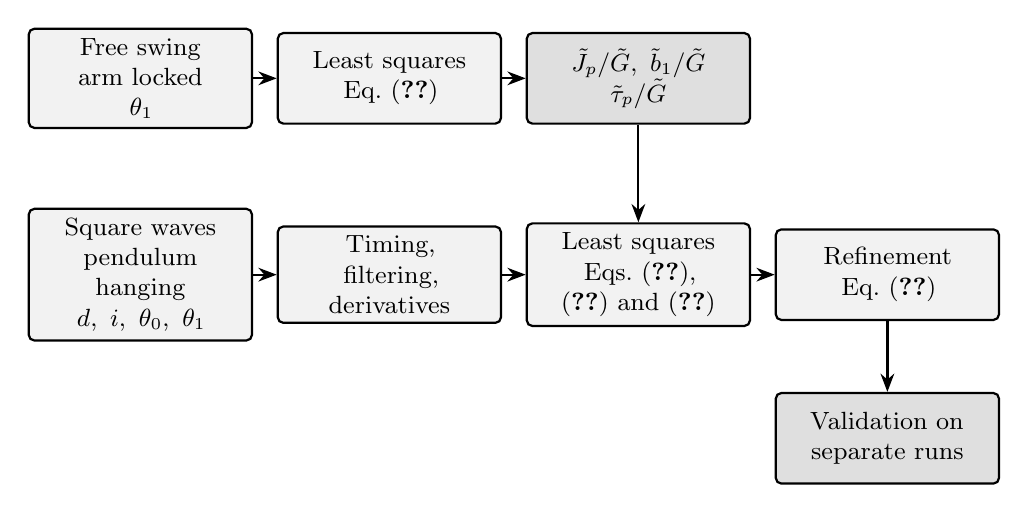
\begin{tikzpicture}[
  box/.style={draw, thick, rounded corners=2pt, fill=gray!10, align=center, font=\small, minimum height=1.15cm, text width=2.6cm},
  res/.style={box, fill=gray!25},
  arr/.style={-{Stealth}, thick},
  node distance=0.3cm]
  \node[box] (sw) {Free swing\\arm locked\\$\theta_1$};
  \node[box, right=of sw] (fsw) {Least squares\\Eq.~\eqref{eq:swing}};
  \node[res, right=of fsw] (psw) {$\tilde J_p/\tilde G,\ \tilde b_1/\tilde G$\\$\tilde\tau_p/\tilde G$};
  \node[box, below=1.0cm of sw] (sq) {Square waves\\pendulum hanging\\$d,\ i,\ \theta_0,\ \theta_1$};
  \node[box, right=of sq] (pr) {Timing,\\filtering,\\derivatives};
  \node[box, right=of pr] (ls) {Least squares\\Eqs.~\eqref{eq:elec_reg},\\\eqref{eq:pend_reg} and~\eqref{eq:arm_reg}};
  \node[box, right=of ls] (oe) {Refinement\\Eq.~\eqref{eq:oe}};
  \node[res, below=0.9cm of oe] (val) {Validation on\\separate runs};
  \draw[arr] (sw) -- (fsw); \draw[arr] (fsw) -- (psw);
  \draw[arr] (sq) -- (pr); \draw[arr] (pr) -- (ls); \draw[arr] (ls) -- (oe); \draw[arr] (oe) -- (val);
  \draw[arr] (psw.south) -- (ls.north);
\end{tikzpicture}
\caption{Parameter estimation procedure used in this work.}
\label{fig:stages}
\end{figure}

\subsection{Experimental Setup}
The experiments were performed on the assembled Furuta pendulum with the instrumentation listed in Table~\ref{tab:setup}.

The microcontroller runs the control loop at 1\,kHz, stores a record every 2\,ms and streams every second record over USB to the desktop application. The application saves the raw encoder counts, the raw pendulum angle, the current-sensor voltage and the applied duty cycle of every sample, together with the device configuration.

The applied duty cycle, rather than the requested one, is used as the input in all fits, so that the slew-rate limit and the short standby at each reversal of the driver are included automatically.

During powered experiments, the firmware limited the arm travel to $\pm 120^\circ$ about the center, the duty cycle to 50\,\% and the filtered current to 1.5\,A, and it stopped the motor if the host heartbeat was lost.

\begin{table}[h]
\centering
\caption{Instrumentation and data acquisition.}
\label{tab:setup}
\small
\begin{tabular}{@{}p{2.6cm}p{6.9cm}p{5.2cm}@{}}
\toprule
Quantity & Sensor / device & Resolution and sampling \\
\midrule
Arm angle $\theta_0$ & 11 PPR quadrature encoder on the motor shaft, $\times 4$, 34:1 gearbox & 1496 counts/rev ($0.24^\circ$) \\
Pendulum angle $\theta_1$ & AS5600 12-bit magnetic encoder (I$^2$C) & $0.088^\circ$, read at 500\,Hz \\
Current $i$ & ACS712-05B (185\,mV/A) on the ESP32-S3 ADC & 2\,kHz, 8 conversions averaged \\
 & on-board 2nd-order Butterworth filter & 40\,Hz cut-off, 5.6\,ms delay \\
Voltage $V$ & TB6612FNG, 20\,kHz PWM, $V = d\,V_s$ & $V_s = 12\,\mathrm{V}$, 10-bit duty \\
Data stream & ESP32-S3 to desktop application & 250\,Hz per channel \\
\bottomrule
\end{tabular}
\end{table}

\subsubsection{Experiments}
The experiments are listed in Table~\ref{tab:runs}. The two free swings were recorded with the arm locked at the center by a rod and the motor unpowered, releasing the pendulum from about $40^\circ$ and $32^\circ$ to opposite sides.

All driven experiments use centered square waves of the duty cycle. Each frequency is applied for a whole number of periods (about 4\,s) with the phase shifted by a quarter period, so that the arm swings symmetrically about its starting angle instead of drifting to one side.

The frequencies were chosen at least 25\,\% away from the natural frequency of the pendulum (1.99\,Hz, see section~\ref{sec:swingresults}). Near resonance, the pendulum swings past horizontal, where the motion becomes strongly nonlinear and a small parameter error changes the response considerably.

The amplitudes of 20--28\,\% duty keep the arm well above the friction level (about 7\,\% duty) while staying inside the travel limit. Three experiments were used for fitting, and three different ones only for validation.

\begin{table}[h]
\centering
\caption{Experiments. The amplitude is the peak duty cycle of the square wave; $|\varphi|_{\max}$ is the largest pendulum angle from hanging and $|i|_{99}$ the 99th percentile of the current magnitude.}
\label{tab:runs}
\small
\begin{tabular}{@{}llllll@{}}
\toprule
Experiment & Amplitude & Frequencies [Hz] & $|\varphi|_{\max}$ & Arm range & $|i|_{99}$ \\
\midrule
Free swing 1, 2 & -- (arm locked) & -- & $40^\circ$, $32^\circ$ & -- & -- \\
Fit 1 & 25\,\% & 1, 1.4, 3.5, 4.5 & $57^\circ$ & $-52^\circ$ to $56^\circ$ & 0.77\,A \\
Fit 2 & 25\,\% & 1, 1.4, 3.5, 4.5 & $53^\circ$ & $-42^\circ$ to $65^\circ$ & 0.77\,A \\
Fit 3 & 20\,\% & 1.2, 2.7, 3.5, 5 & $27^\circ$ & $-1^\circ$ to $22^\circ$ & 0.63\,A \\
Validation 1 & 22\,\% & 1.1, 3, 4 & $51^\circ$ & $-42^\circ$ to $39^\circ$ & 0.69\,A \\
Validation 2 & 28\,\% & 1.3, 2.6, 3.8, 5 & $86^\circ$ & $-41^\circ$ to $52^\circ$ & 0.83\,A \\
Validation 3 & 24\,\% & 0.9, 1.5, 3.3, 4.2 & $64^\circ$ & $-46^\circ$ to $67^\circ$ & 0.76\,A \\
\bottomrule
\end{tabular}
\end{table}

Four further experiments were recorded but not used in the final fit:
\begin{enumerate}
  \item A run near resonance (20\,\% at 1.8, 2.2 and 2.7\,Hz) swung the pendulum to $104^\circ$. Including it shifted the coupling $\tilde h$ in the opposite direction to the simulation-error refinement and lowered the pendulum fit of the validation runs, so it was left out.
  \item Two runs at 30\,\% and 15\,\% duty extended the speed range of the arm, which exposed the shape of the arm friction discussed in section~\ref{sec:lsresults}.
  \item A stall test, with the arm locked by the rod and duty steps of $\pm 6$ to $\pm 15$\,\%, measured the resistance at standstill and the play between the motor shaft and the arm.
\end{enumerate}

\subsection{Signal Processing}
\label{sec:processing}
Each channel carries its own timestamp (encoder, pendulum sensor and ADC), and every recording is resampled onto a uniform grid at the median sample interval of 4\,ms, using the longest stretch without missing or invalid samples.

The applied duty cycle is held constant between samples, so that the zero-duty samples stay exactly zero. The 5.6\,ms delay of the on-board current filter is removed by shifting the current timestamps.

The same zero-phase second-order Butterworth low-pass filter, with a cut-off of $f_d = 40\,\mathrm{Hz}$, is then applied to every signal, and the velocities and accelerations are obtained by central differences.

Since the nonlinear regressors (for example $\sgn(\dot\theta_0)$ or $\sin\theta_1\,\dot\theta_1^2$) are formed after this step, both sides of every regression are filtered again with a common zero-phase low-pass filter at $f_p = 10\,\mathrm{Hz}$ and decimated to $4 f_p$, so that the residuals are closer to white.

Samples near the ends of a recording, samples at zero duty (for equation~\ref{eq:elec_reg}) and samples where the arm is stuck or slower than $\omega_{\min}$ (for equation~\ref{eq:arm_reg}) are excluded from the corresponding regression.

The choice of the two cut-offs was checked with a grid of $f_d \in \{15, 20, 30, 40, 60\}\,\mathrm{Hz}$ and $f_p \in \{4, 6, 8, 10, 15\}\,\mathrm{Hz}$, by scoring each identified model on the validation runs. All combinations with $f_p \le 10\,\mathrm{Hz}$ gave practically the same validation fit (within 0.6 percentage points), while $f_p = 15\,\mathrm{Hz}$ was 1 to 1.5 points worse. Thus, the filters do not limit the accuracy, and $f_d = 40\,\mathrm{Hz}$ with $f_p = 10\,\mathrm{Hz}$ is kept.

\subsubsection{Pendulum Timing Correction}
When equation~\ref{eq:pend_reg} is fitted, the pendulum angle is found to lag the arm and current signals.

To find this lag, the pendulum timestamps were shifted earlier by a trial delay and the fit was repeated, which gives the coefficient of determination of Figure~\ref{fig:delay}. It peaks between 7 and 8\,ms and changes by less than 0.3\,\% between 6 and 9\,ms, so a correction of 7\,ms is used.

The lag may come from the internal filter of the AS5600 or from the arm lagging the motor shaft through the gearbox play. In both cases, a fixed time shift accounts for it.

\begin{figure}[h]
\centering
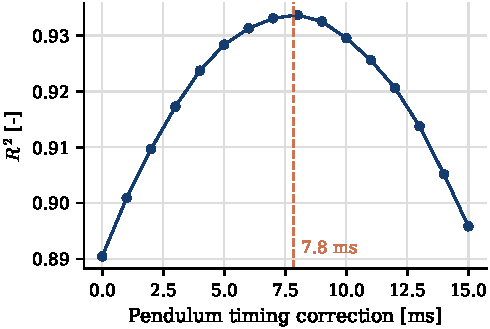
\includegraphics[width=0.55\textwidth]{figures/fig_delay.pdf}
\caption{Coefficient of determination of the pendulum equation~\eqref{eq:pend_reg} on the three fit runs against the timing correction of the pendulum angle.}
\label{fig:delay}
\end{figure}

\subsection{Free-Swing Results}
\label{sec:swingresults}
Fitting equation~\ref{eq:swing} to the two free swings gave the values of Table~\ref{tab:swing}. The samples before the release, while the pendulum was held or lifted by hand, are excluded automatically by detecting where the pendulum is displaced but not moving.

The two swings agree within 0.1\,\% in $\tilde J_p/\tilde G$ and in the natural frequency, and the arm encoder did not change by a single count in either of them, which is a good indication that the rod held the arm still.

Including the dry-friction term raises the coefficient of determination from 0.9907 to 0.9924 (a value of one means a perfect fit), and Figure~\ref{fig:swing} shows that the fitted model follows the measured swing over its whole decay.

\begin{table}[h]
\centering
\caption{Free-swing results (both swings fitted together).}
\label{tab:swing}
\small
\begin{tabular}{@{}lll@{}}
\toprule
Quantity & Value & Note \\
\midrule
$\tilde J_p/\tilde G$ & $6.393\times10^{-3}\,\mathrm{s^2}$ & $\pm0.2\,\%$; swings: $6.390$, $6.396\times10^{-3}$ \\
$\tilde b_1/\tilde G$ & $3.78\times10^{-3}\,\mathrm{s}$ & $\pm7\,\%$ \\
$\tilde\tau_p/\tilde G$ & $0.0174\,\mathrm{rad}$ ($1.0^\circ$) & $\pm5\,\%$; amplitude loss $2.0^\circ$ per half period \\
$\omega_n$ & $12.51\,\mathrm{rad/s}$ ($1.99\,\mathrm{Hz}$) & swings: 12.510 and 12.504\,rad/s \\
$\zeta$ (viscous part) & 0.024 & \\
Equivalent length $g\,\tilde J_p/\tilde G$ & 6.27\,cm & \\
\bottomrule
\end{tabular}
\end{table}

\begin{figure}[h]
\centering
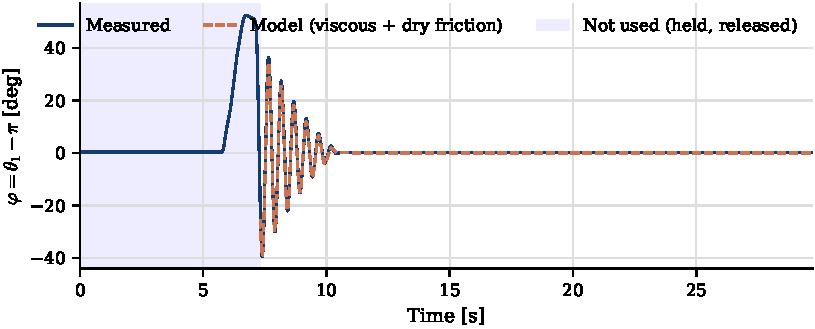
\includegraphics[width=\textwidth]{figures/fig_swing.pdf}
\caption{Measured free swing (released from $40^\circ$) and the simulated swing of Eq.~\eqref{eq:swing} with the fitted viscous and dry friction. The shaded interval, before the release, is not used in the fit.}
\label{fig:swing}
\end{figure}

\subsection{Least-Squares Results}
\label{sec:lsresults}

\subsubsection{Electrical Parameters}
Equation~\ref{eq:elec_reg} fitted on 911 driven samples of the three fit runs gives \textbf{\boldmath$R_m = 3.425\,\Omega$} and \textbf{\boldmath$K_b = 0.4814\,\mathrm{V\,s/rad}$}, with a coefficient of determination of 0.995. With $V$ on the left-hand side instead, $R_m = 3.387\,\Omega$ and $K_b = 0.4848\,\mathrm{V\,s/rad}$.

Fitted run by run, $R_m$ varies between 3.34 and 3.83\,$\Omega$ and $K_b$ between 0.42 and 0.50\,V\,s/rad. This is because in a square-wave run the voltage and the speed rise and fall together, which makes the two regressors of equation~\ref{eq:elec_reg} partly collinear. Pooling the three runs averages this out.

The stall test measured $V/i$ directly, since there is no back-EMF at standstill, and gave $4.13\,\Omega$. The higher resistance at standstill is expected for a brushed motor, where the brush contact resistance depends on the rotor position and on the commutation. Therefore, the value obtained during motion is the one that describes the running motor.

\subsubsection{Pendulum Coupling}
Fitting equation~\ref{eq:pend_reg} with the free-swing ratios fixed gives \textbf{\boldmath$\tilde h/\tilde G = 6.22\times10^{-3}\,\mathrm{s^2}$} on 1820 samples, with a coefficient of determination of the whole equation of 0.933. By equation~\ref{eq:Larm}, this corresponds to an arm length of \textbf{6.10\,cm}.

\subsubsection{Arm Parameters}
Equation~\ref{eq:arm_reg} gives \textbf{\boldmath$\tilde J_a = 5.634\times10^{-3}\,\mathrm{A\,s^2/rad}$}, \textbf{\boldmath$\tilde G = 0.0290\,\mathrm{A}$}, \textbf{\boldmath$\tilde B_{eq} = 0.0161\,\mathrm{A\,s/rad}$}, \textbf{\boldmath$\tilde\tau_{c+} = 0.258\,\mathrm{A}$} and \textbf{\boldmath$\tilde\tau_{c-} = 0.257\,\mathrm{A}$}, with a coefficient of determination of 0.995.

The pendulum reaction $\tilde G\, T_r$ is only a few percent of the arm equation, so $\tilde G$ is the least certain of these values ($\pm 9\,\%$). As shown in section~\ref{sec:stability}, this matters little, since the dynamics depend on $\tilde G$ mainly through the coupling ratio $\tilde h^2/(\tilde J_a \tilde J_p)$, which is only about 4\,\%.

\subsubsection{Shape of the Arm Friction}
To check the friction model, the inertial and pendulum terms were subtracted from the measured current, which leaves the friction current. It is plotted against the arm speed in Figure~\ref{fig:friction} for all driven experiments.

Above about 2\,rad/s, the friction is almost constant at 0.30--0.32\,A and even decreases slightly at the highest speeds, while the model $\tilde\tau_c + \tilde B_{eq}\dot\theta_0$ keeps rising.

At low speed, the plotted values are smeared by the filtering during the fast reversals of the square wave, and the slow 15\,\% experiment shows that the friction there is already about 0.27\,A.

Thus, the friction of this gearmotor behaves like Coulomb friction with very little viscous part, and the straight line of the model is a fit over the speed range of the experiments. This explains why the 30\,\% experiment, which reaches 6\,rad/s, gives different friction values (and a negative $\tilde G$) when it is added to the fit, and it is the reason why the fit and validation experiments were kept at 20--28\,\% duty.

\begin{figure}[h]
\centering
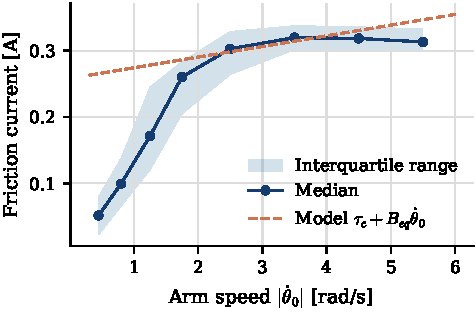
\includegraphics[width=0.55\textwidth]{figures/fig_friction.pdf}
\caption{Friction current of the arm against the arm speed, for all driven experiments, compared with the identified linear friction model.}
\label{fig:friction}
\end{figure}

\subsection{Refinement Results}
Refining $\tilde h$, $\tilde b_1$ and $\tilde\tau_p$ with equation~\ref{eq:oe} on nine 4\,s windows of the fit runs reduced the cost from 336 to 270 and changed the three parameters by $+11.6\,\%$, $+10.3\,\%$ and $+26.3\,\%$.

The increase of $\tilde h$ is the expected correction of the errors-in-variables bias previously discussed in section~\ref{sec:estmodels}, and the corrected coupling gives an arm length of \textbf{6.81\,cm}.

The increase of the pendulum damping shows that the pendulum is damped more strongly while the arm moves than in the free swing with the arm locked.

The arm parameters were also tried as refinement variables. However, refining the friction terms traded the open-loop drift of the arm between the validation runs rather than reducing it (see Table~\ref{tab:variants}), so they are kept at their least-squares values.

\subsection{Validation}
To measure how closely our model reproduces the hardware, the identified model (equation~\ref{eq:scaled}) was simulated with the recorded duty cycle of each validation run, starting from the measured state, and compared with the measured signals. The agreement is expressed as the fit percentage
\begin{equation}
  \mathrm{fit} = 100 \left(1 - \frac{\lVert \mathbf{y} - \hat{\mathbf{y}} \rVert}{\lVert \mathbf{y} - \bar y \rVert}\right)\ \%,
\end{equation}
where $\mathbf{y}$ is the measured signal, $\hat{\mathbf{y}}$ the simulated one and $\bar y$ the mean of the measurement (100\,\% means a perfect match, 0\,\% means no better than a constant).

Two simulations are used. The first is an open-loop simulation over the whole run of about 15\,s. The second restarts from the measured state every 2\,s, which shows the short-term accuracy that matters for a controller.

Table~\ref{tab:validation} gives the results of the final model, and Figure~\ref{fig:validation} compares the open-loop simulation with the measurements for the first and third validation runs.

\begin{table}[h]
\centering
\caption{Validation of the final model on the three validation runs (fit percentage; RMS error of the open-loop simulation in brackets).}
\label{tab:validation}
\small
\begin{tabular}{@{}lccc@{}}
\toprule
 & Validation 1 & Validation 2 & Validation 3 \\
\midrule
Pendulum angle, open loop & 90\,\% ($1.4^\circ$) & 84\,\% ($3.3^\circ$) & 85\,\% ($2.9^\circ$) \\
Pendulum angle, restarted every 2\,s & 90\,\% & 86\,\% & 88\,\% \\
Arm angle, restarted every 2\,s & 88\,\% & 86\,\% & 86\,\% \\
Arm angle, open loop & 89\,\% ($1.5^\circ$) & $-3$\,\% ($16.7^\circ$) & 42\,\% ($11.3^\circ$) \\
Arm speed, open loop & 92\,\% & 93\,\% & 90\,\% \\
Current, open loop & 88\,\% (0.043\,A) & 89\,\% (0.049\,A) & 88\,\% (0.048\,A) \\
\bottomrule
\end{tabular}
\end{table}

\begin{figure}[h]
\centering
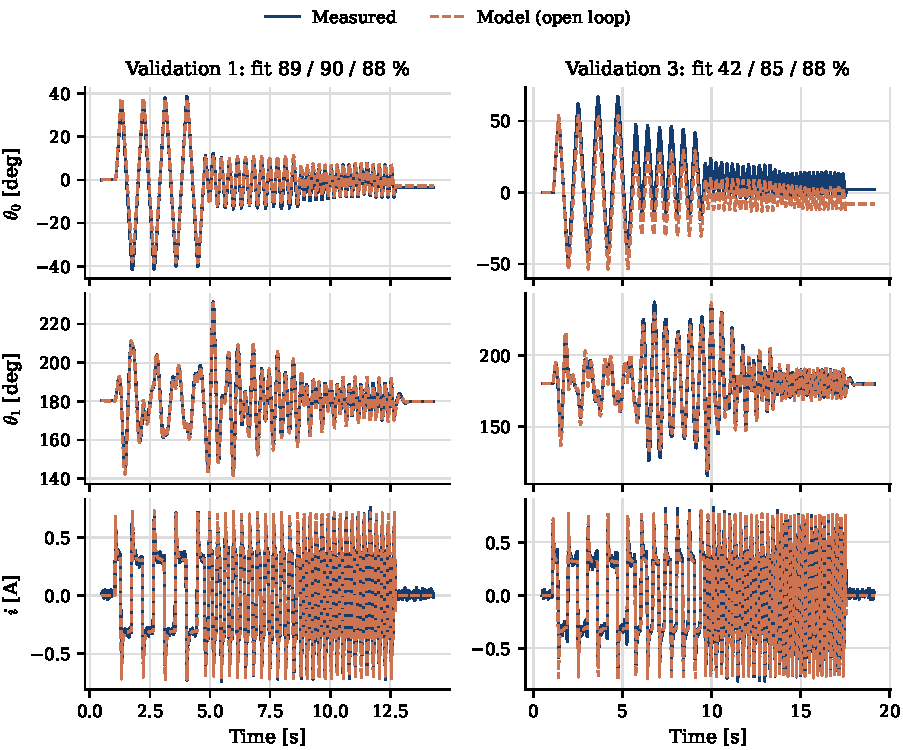
\includegraphics[width=\textwidth]{figures/fig_validation.pdf}
\caption{Measured arm angle, pendulum angle and current of validation runs 1 and 3 compared with the open-loop simulation of the final model driven by the recorded duty cycle. The titles give the fit of the arm angle, the pendulum angle and the current.}
\label{fig:validation}
\end{figure}

The pendulum angle, the arm speed and the current are reproduced closely in all three runs, including the third one, which was recorded after every modeling choice had been made. The current is limited to about 88\,\% by the noise of the current sensor itself.

The open-loop arm angle is the only quantity that varies strongly between runs, from 89\,\% to $-3$\,\%. Since the arm angle is the integral of the arm speed, a small difference between the friction in the two directions makes it drift steadily over a 15\,s simulation. Shifting the current zero by only 0.02\,A, which changes that balance, reduced the arm-angle fit to about 50\,\% even with restarts every 2\,s.

Restarting every 2\,s removes the drift and gives \textbf{86--88\,\%} for the arm angle in every run. A feedback controller corrects a slow drift of this kind, so the short-term accuracy is the relevant measure for controller design.

Table~\ref{tab:variants} compares the least-squares model with the refinement variants. Refining $\tilde h$ alone improves the pendulum, and refining the pendulum damping as well improves it further in every run. Refining all nine parameters gives a similar pendulum fit, but it moves the open-loop arm drift from one run to another. Therefore, the variant with $\tilde h$, $\tilde b_1$ and $\tilde\tau_p$ refined is taken as the final model.

\begin{table}[h]
\centering
\caption{Comparison of the estimation variants on validation runs 1 / 2 / 3 (fit percentage).}
\label{tab:variants}
\small
\begin{tabular}{@{}lcccc@{}}
\toprule
Variant & Pendulum, open loop & Pendulum, 2\,s & Arm, 2\,s & Arm, open loop \\
\midrule
Least squares only & 86 / 73 / 77 & 86 / 76 / 81 & 88 / 86 / 86 & 89 / $-3$ / 42 \\
Refined $\tilde h$ & 86 / 80 / 82 & 88 / 83 / 85 & 88 / 86 / 86 & 89 / $-3$ / 42 \\
\textbf{Refined $\tilde h$, $\tilde b_1$, $\tilde\tau_p$} & \textbf{90 / 84 / 85} & \textbf{90 / 86 / 88} & \textbf{88 / 86 / 86} & \textbf{89 / $-3$ / 42} \\
Refined, nine parameters & 91 / 87 / 84 & 91 / 86 / 87 & 88 / 88 / 85 & 38 / 57 / 66 \\
\bottomrule
\end{tabular}
\end{table}

Several other methods were tested in the same way and did not improve the validation fit:
\begin{enumerate}
  \item placing the voltage instead of the current on the left-hand side of the arm equation, which only exchanged viscous for Coulomb friction;
  \item adding a constant voltage drop of the driver to equation~\ref{eq:qs}, which was fitted as 0.14\,V;
  \item fixing $R_m$ at the standstill value of 4.1\,$\Omega$;
  \item replacing the Coulomb friction by a smooth saturating function of the speed.
\end{enumerate}

\subsection{Identified Parameters}
The final parameters of our system are listed in Table~\ref{tab:params}.

\begin{table}[h]
\centering
\caption{Identified parameters of the final model. The uncertainty is the approximate relative standard error of the least-squares fit; the parameters marked $^*$ were refined by simulation error, and their least-squares values are given in the last column.}
\label{tab:params}
\small
\begin{tabular}{@{}llllll@{}}
\toprule
Parameter & Value & Unit & Uncertainty & Description & Least squares \\
\midrule
$R_m$ & 3.425 & $\Omega$ & 0.4\,\% & armature resistance (incl. driver) & \\
$K_b$ & 0.4814 & V\,s/rad & 0.3\,\% & back-EMF constant (arm shaft) & \\
$\tilde J_a$ & $5.634\times10^{-3}$ & A\,s$^2$/rad & 0.4\,\% & arm-side inertia & \\
$\tilde J_p$ & $1.853\times10^{-4}$ & A\,s$^2$/rad & 9\,\% & pendulum inertia about its pivot & \\
$\tilde h^*$ & $2.012\times10^{-4}$ & A\,s$^2$/rad & 8\,\% & inertial coupling & $1.804\times10^{-4}$ \\
$\tilde G$ & $2.899\times10^{-2}$ & A & 9\,\% & gravity torque coefficient & \\
$\tilde B_{eq}$ & $1.612\times10^{-2}$ & A\,s/rad & 7\,\% & arm viscous friction & \\
$\tilde b_1^*$ & $1.208\times10^{-4}$ & A\,s/rad & 11\,\% & pendulum viscous friction & $1.095\times10^{-4}$ \\
$\tilde\tau_{c+}$ & 0.2581 & A & 1.3\,\% & arm Coulomb friction, $\dot\theta_0>0$ & \\
$\tilde\tau_{c-}$ & 0.2569 & A & 1.3\,\% & arm Coulomb friction, $\dot\theta_0<0$ & \\
$\tilde\tau_p^*$ & $6.38\times10^{-4}$ & A & 8\,\% & pendulum joint dry friction & $5.05\times10^{-4}$ \\
\midrule
$\La$ & 6.81 & cm & & arm length, Eq.~\eqref{eq:Larm} & 6.10 \\
$t_d$ & 7 & ms & & pendulum timing correction & \\
\bottomrule
\end{tabular}
\end{table}

In terms of the duty cycle, the Coulomb friction corresponds to $R_m \tilde\tau_{c\pm}/V_s = 7.4\,\%$ and $7.3\,\%$, which is the friction compensation previously described in section~\ref{sec:full}.

The back-EMF damping $K_b/R_m = 0.141\,\mathrm{A\,s/rad}$ is almost nine times the mechanical viscous friction $\tilde B_{eq}$, so the damping of the arm is set mainly by the motor.

\subsection{Limitations}
Limitations of the presented model and estimation are:
\begin{enumerate}
  \item The torque scale is not identified:
  \begin{enumerate}
    \item the torque constant, and with it the gearbox efficiency and the inertias in $\mathrm{kg\,m^2}$, cannot be obtained from the measured signals;
    \item the model is complete in terms of current and voltage, but physical torques require one absolute reference such as a known added mass.
  \end{enumerate}
  \item The friction model is a straight line:
  \begin{enumerate}
    \item it is modeled as Coulomb plus viscous friction, which fits the speed range of the experiments (up to about 5\,rad/s);
    \item at higher speeds the friction stays constant, so the model overestimates it there.
  \end{enumerate}
  \item The open-loop arm angle drifts over long simulations because of the small run-to-run variation of the friction in the two directions (see Table~\ref{tab:validation}).
  \item The gearbox play, felt by hand to be below $2^\circ$ at the arm, is not modeled. It may contribute to the slightly overestimated pendulum response at the highest excitation frequencies.
  \item The inductance was not identified, so the reduced four-state model is used. This is justified only while the closed-loop poles stay well below the electrical pole.
  \item Swings close to horizontal (Validation 2 reached $86^\circ$) are reproduced less accurately than moderate swings.
\end{enumerate}

%======================================================================
\section{Identified State-Space Models}
\label{sec:ssmodels}
%======================================================================
Substituting the parameters of Table~\ref{tab:params} into equations~\ref{eq:beta} to~\ref{eq:outputs} gives the numerical linear models of our system, which are the starting point for the controller design. The nonlinear model used for simulation follows in section~\ref{sec:nlmodel}. The angles are in radians, the voltage in volts, the duty cycle as a fraction $d \in [-1, 1]$ and the current in amperes.

\subsection{Upright Equilibrium}
With $\mathbf{x} = \begin{bmatrix} \theta_0 & \theta_1 & \dot\theta_0 & \dot\theta_1 \end{bmatrix}^T$,
\begin{equation}
\boxed{
\begin{aligned}
  \dot{\mathbf{x}} &= A_4 \mathbf{x} + B_4 V, &
  A_4 &= \begin{bmatrix}
  0 & 0 & 1 & 0\\
  0 & 0 & 0 & 1\\
  0 & -5.812 & -28.92 & 0.0242\\
  0 & 162.7 & 31.41 & -0.678
  \end{bmatrix}, &
  B_4 &= \begin{bmatrix} 0 \\ 0 \\ 53.90 \\ -58.53 \end{bmatrix},\\[4pt]
  \mathbf{y} &= C\mathbf{x} + D V, &
  C &= \begin{bmatrix} 1 & 0 & 0 & 0 \\ 0 & 1 & 0 & 0 \\ 0 & 0 & -0.1405 & 0 \end{bmatrix}, &
  D &= \begin{bmatrix} 0 \\ 0 \\ 0.2919 \end{bmatrix}.
\end{aligned}
}
\label{eq:ss_up_num}
\end{equation}
With the duty cycle as input, $B_d = V_s B_4 = \begin{bmatrix} 0 & 0 & 646.8 & -702.4 \end{bmatrix}^T$ and $D_d = \begin{bmatrix} 0 & 0 & 3.503 \end{bmatrix}^T$.

The transfer functions from the voltage to the two angles are
\begin{equation}
  \frac{\Theta_0(s)}{V(s)} = \frac{53.90\,(s + 12.84)(s - 12.19)}{s\,(s - 12.26)(s + 12.63)(s + 29.23)}, \qquad
  \frac{\Theta_1(s)}{V(s)} = \frac{-58.53\, s}{(s - 12.26)(s + 12.63)(s + 29.23)} ,
  \label{eq:tf_up}
\end{equation}
where the common factor $s$ of $\Theta_1/V$ has been cancelled. This can be intuitively understood since a constant voltage drives the arm at a constant speed, which leaves the pendulum angle unchanged in steady state.

\subsection{Hanging Equilibrium}
With $\mathbf{x} = \begin{bmatrix} \theta_0 & \varphi & \dot\theta_0 & \dot\varphi \end{bmatrix}^T$ and the same $C$ and $D$,
\begin{equation}
\boxed{
  A_h = \begin{bmatrix}
  0 & 0 & 1 & 0\\
  0 & 0 & 0 & 1\\
  0 & -5.812 & -28.92 & -0.0242\\
  0 & -162.7 & -31.41 & -0.678
  \end{bmatrix}, \qquad
  B_h = \begin{bmatrix} 0 \\ 0 \\ 53.90 \\ 58.53 \end{bmatrix}
}
\label{eq:ss_hang_num}
\end{equation}
and
\begin{equation}
  \frac{\Theta_0(s)}{V(s)} = \frac{53.90\,(s^2 + 0.652\, s + 156.4)}{s\,(s + 28.76)(s^2 + 0.844\, s + 157.3)}, \qquad
  \frac{\Phi(s)}{V(s)} = \frac{58.53\, s}{(s + 28.76)(s^2 + 0.844\, s + 157.3)} .
  \label{eq:tf_hang}
\end{equation}

\subsection{Nonlinear Model}
\label{sec:nlmodel}
The linear models above are only valid for small deviations from an equilibrium. Since the swing-up, large pendulum swings, the friction band of the arm and the switching of the driver at zero duty all lie outside that range, the nonlinear model is needed for simulation in Simulink and for the digital twin.

This is the model that was simulated in the validation of section~\ref{sec:estimation} (see Table~\ref{tab:validation}). It is obtained by substituting the parameters of Table~\ref{tab:params} into equation~\ref{eq:scaled}, with the inductance neglected (equation~\ref{eq:qs}) and the sign functions replaced by the smooth functions of section~\ref{sec:full}.

With the state $\mathbf{x} = \begin{bmatrix} \theta_0 & \theta_1 & \dot\theta_0 & \dot\theta_1 \end{bmatrix}^T$, where $\theta_1 = 0$ is upright and $\theta_1 = \pi$ is hanging, and the duty cycle $d$ as input, the armature current is
\begin{equation}
  i = \begin{cases} \dfrac{12\, d - 0.4814\, \dot\theta_0}{3.425} & d \neq 0 \\[6pt] 0 & d = 0 \end{cases}
  \label{eq:nl_current}
\end{equation}
where $12\,d$ is the armature voltage $V$ in volts. The friction torque of the arm is
\begin{equation}
  \tilde\tau_c(\dot\theta_0) = \begin{cases} 0.2581 \tanh\left(\dot\theta_0 / 0.1\right) & \dot\theta_0 > 0 \\ 0.2569 \tanh\left(\dot\theta_0 / 0.1\right) & \dot\theta_0 \le 0 \end{cases}
  \label{eq:nl_friction}
\end{equation}
in amperes, with $\dot\theta_0$ in rad/s.

By collecting all terms that do not contain an acceleration on the right-hand side of equation~\ref{eq:scaled}, the two mechanical equations become
\begin{equation}
\begin{aligned}
  f_0 = {}& i - 0.01612\,\dot\theta_0 - \tilde\tau_c(\dot\theta_0)\\
  & - 3.706\times10^{-4} \sin\theta_1 \cos\theta_1\, \dot\theta_0 \dot\theta_1 + 2.012\times10^{-4} \sin\theta_1\, \dot\theta_1^2 ,\\[2pt]
  f_1 = {}& 1.853\times10^{-4} \sin\theta_1 \cos\theta_1\, \dot\theta_0^2 - 1.208\times10^{-4}\, \dot\theta_1\\
  & - 6.38\times10^{-4} \tanh\left(\dot\theta_1 / 0.05\right) + 0.02899 \sin\theta_1 ,
\end{aligned}
\label{eq:nl_f}
\end{equation}
so that
\begin{equation}
  \begin{bmatrix} 5.634\times10^{-3} + 1.853\times10^{-4} \sin^2\theta_1 & 2.012\times10^{-4} \cos\theta_1 \\ 2.012\times10^{-4} \cos\theta_1 & 1.853\times10^{-4} \end{bmatrix}
  \begin{bmatrix} \ddot\theta_0 \\ \ddot\theta_1 \end{bmatrix}
  = \begin{bmatrix} f_0 \\ f_1 \end{bmatrix}.
  \label{eq:nl_mass}
\end{equation}
The determinant of this mass matrix is
\begin{equation}
  \delta(\theta_1) = 1.0441\times10^{-6} + 3.434\times10^{-8} \sin^2\theta_1 - 4.049\times10^{-8} \cos^2\theta_1 \ \ge\ 1.0036\times10^{-6} ,
\end{equation}
which is positive for every pendulum angle, so the mass matrix can always be inverted. Inverting it gives the nonlinear state equations of our system:
\begin{equation}
\therefore\;\boxed{
\begin{aligned}
  \dot x_1 &= \dot\theta_0, \qquad \dot x_2 = \dot\theta_1,\\
  \dot x_3 &= \frac{1.853\times10^{-4}\, f_0 - 2.012\times10^{-4} \cos\theta_1\, f_1}{\delta(\theta_1)},\\
  \dot x_4 &= \frac{-2.012\times10^{-4} \cos\theta_1\, f_0 + \left(5.634\times10^{-3} + 1.853\times10^{-4} \sin^2\theta_1\right) f_1}{\delta(\theta_1)}
\end{aligned}
}
\label{eq:nl_num}
\end{equation}
with the outputs $\theta_0$, $\theta_1$ and $i$ (equation~\ref{eq:nl_current}).

Linearizing equation~\ref{eq:nl_num} about $\theta_1 = 0$ or $\theta_1 = \pi$, with the friction left out, gives back the matrices of equations~\ref{eq:ss_up_num} and~\ref{eq:ss_hang_num}, which is a good check of the consistency of the two forms.

In Simulink, equation~\ref{eq:nl_num} can be implemented with a MATLAB Function block that evaluates the state derivative and the current, followed by an integrator for the four states, with the initial condition $\mathbf{x}(0) = \begin{bmatrix} 0 & \pi & 0 & 0 \end{bmatrix}^T$ for a pendulum hanging at rest. The validation simulations used a fourth-order Runge--Kutta method with a step of 2\,ms, so a fixed step of 2\,ms or smaller (or a variable-step solver) should be used to reproduce them.

%======================================================================
\section{Stability Analysis}
\label{sec:stability}
%======================================================================
To decide whether our system needs feedback to stay at an equilibrium, its open-loop stability is checked through the eigenvalues of the system matrix, which are the poles of the linear model.

An equilibrium is asymptotically stable if every eigenvalue of $A$ has a negative real part, and unstable if at least one eigenvalue has a positive real part. The eigenvalues are the roots of the characteristic equation
\begin{equation}
  \det\left(sI - A\right) = 0 .
\end{equation}

\subsection{Upright Equilibrium}
For $A_4$ of equation~\ref{eq:ss_up_num}, the characteristic equation is
\begin{equation}
  s^4 + 29.60\, s^3 - 143.9\, s^2 - 4525\, s = s\,(s - 12.26)(s + 12.63)(s + 29.23) = 0 .
  \label{eq:char_up}
\end{equation}
Since two coefficients of the characteristic polynomial are negative, the Routh--Hurwitz criterion already shows that at least one root lies in the right half-plane, and the factorization confirms it. The four poles are interpreted in Table~\ref{tab:poles_up}.

\begin{table}[h]
\centering
\caption{Poles of the upright model.}
\label{tab:poles_up}
\small
\begin{tabular}{@{}lll@{}}
\toprule
Pole [rad/s] & Time constant & Meaning \\
\midrule
$+12.26$ & 81.6\,ms (growth) & the pendulum falls; a deviation grows by a factor $e$ every 82\,ms \\
$0$ & -- & arm angle; no restoring torque acts on it (neutrally stable) \\
$-12.63$ & 79.2\,ms & stable mirror of the falling mode \\
$-29.23$ & 34.2\,ms & arm motion damped by the back-EMF and friction \\
\bottomrule
\end{tabular}
\end{table}

Since the pole at \textbf{\boldmath$+12.26\,\mathrm{rad/s}$} lies in the right half-plane, the upright equilibrium is unstable in open loop, as expected for an inverted pendulum, and it must be stabilized by feedback.

For comparison, an inverted pendulum on a fixed arm would have its poles at $\pm\sqrt{\tilde G/\tilde J_p} = \pm 12.51\,\mathrm{rad/s}$, the same magnitude as the measured natural frequency of the hanging pendulum. The free arm moves the unstable pole slightly to $12.26\,\mathrm{rad/s}$ through the inertial coupling and the damping, which agrees with what we would expect from equation~\ref{eq:lin}.

This pole sets the minimum speed of any stabilizing controller, since the closed loop must react considerably faster than the 82\,ms time constant of the fall.

The controllability matrix $\begin{bmatrix} B_4 & A_4 B_4 & A_4^2 B_4 & A_4^3 B_4 \end{bmatrix}$ has full rank (4), so all four poles can be placed by state feedback. The observability matrix built from the two encoder outputs $\theta_0$ and $\theta_1$ alone also has full rank (4), so the velocities can be estimated by an observer.

Furthermore, $\Theta_0/V$ in equation~\ref{eq:tf_up} has a zero at $s = +12.19\,\mathrm{rad/s}$ in the right half-plane. This non-minimum-phase zero limits the bandwidth that can be achieved by a loop closed on the arm angle alone.

Moreover, the two zeros of $\Theta_0/V$ ($+12.19$ and $-12.84\,\mathrm{rad/s}$) lie close to the two pendulum poles ($+12.26$ and $-12.63\,\mathrm{rad/s}$), as can be seen in Figure~\ref{fig:pz}. This near cancellation means that the falling mode of the pendulum is barely visible in the arm angle, so a stabilizing controller has to feed back the pendulum angle measured by the AS5600 and cannot rely on the arm encoder alone.

\subsection{Hanging Equilibrium}
For $A_h$ of equation~\ref{eq:ss_hang_num},
\begin{equation}
  s^4 + 29.60\, s^3 + 181.6\, s^2 + 4525\, s = s\,(s + 28.76)(s^2 + 0.844\, s + 157.3) = 0 ,
  \label{eq:char_hang}
\end{equation}
with poles at $0$, $-28.76$ and $-0.422 \pm 12.54j\,\mathrm{rad/s}$.

The complex pair is the pendulum swing, with a natural frequency of \textbf{\boldmath$\sqrt{157.3} = 12.54\,\mathrm{rad/s}$} (2.00\,Hz) and a damping ratio of $0.422/12.54 = 0.034$. The frequency agrees with the free swing of section~\ref{sec:swingresults} (12.51\,rad/s) within 0.3\,\%, which is a good indication of the consistency of the identified parameters.

The damping is higher than the free-swing value of 0.024, because the swinging pendulum now also moves the free arm, whose motion is damped by the back-EMF.

All poles except the arm-angle pole at the origin lie in the left half-plane, so the hanging equilibrium is stable in the sense that any pendulum swing decays, while the arm can come to rest at any angle. The pole-zero maps of both equilibria are shown in Figure~\ref{fig:pz}.

\begin{figure}[h]
\centering
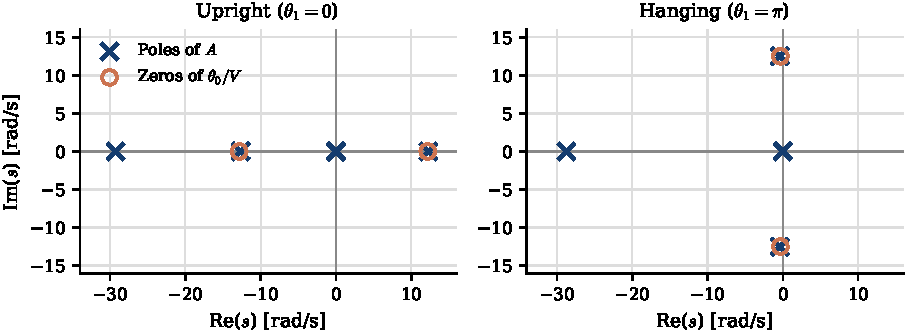
\includegraphics[width=\textwidth]{figures/fig_pz.pdf}
\caption{Poles of the identified system matrices and zeros of $\Theta_0(s)/V(s)$ for the upright and hanging equilibria. In both cases two zeros lie next to the poles of the pendulum mode.}
\label{fig:pz}
\end{figure}

\subsection{Validity of the Reduced Model}
The linear models leave out the friction terms, so they describe motions in which the arm keeps moving. Inside the friction band of about 7\,\% duty the arm sticks, which a linear model cannot represent and which a controller can compensate as previously described in section~\ref{sec:full}.

The models also neglect the inductance. With an electrical time constant of the order of a millisecond (see section~\ref{sec:estmodels}), the neglected electrical pole lies near $-1000\,\mathrm{rad/s}$, more than thirty times faster than the fastest mechanical pole of $-29.2\,\mathrm{rad/s}$.

Thus, the four-state models of section~\ref{sec:ssmodels} are suitable for controller design as long as the closed-loop poles remain well below this value.

\end{document}
